% $Header: /Users/joseph/Documents/LaTeX/beamer/solutions/conference-talks/conference-ornate-20min.en.tex,v 90e850259b8b 2007/01/28 20:48:30 tantau $

\documentclass{beamer}

% This file is a solution template for:

% - Talk at a conference/colloquium.
% - Talk length is about 20min.
% - Style is ornate.



% Copyright 2004 by Till Tantau <tantau@users.sourceforge.net>.
%
% In principle, this file can be redistributed and/or modified under
% the terms of the GNU Public License, version 2.
%
% However, this file is supposed to be a template to be modified
% for your own needs. For this reason, if you use this file as a
% template and not specifically distribute it as part of a another
% package/program, I grant the extra permission to freely copy and
% modify this file as you see fit and even to delete this copyright
% notice. 


\mode<presentation>
{
  \usetheme{default}
  % or ...

  \setbeamercovered{transparent}
  % or whatever (possibly just delete it)
}


\usepackage[english]{babel}
% or whatever

\usepackage[latin1]{inputenc}
% or whatever

\usepackage{times}
\usepackage[T1]{fontenc}
% Or whatever. Note that the encoding and the font should match. If T1
% does not look nice, try deleting the line with the fontenc.

\usepackage{epstopdf,chemfig}
\usepackage{xcolor}
\DeclareMathOperator*{\argmin}{arg\,min}
\newenvironment{greyedout}{\color{gray}}{\ignorespacesafterend}
\setbeamercolor{alerted text}{fg = red}


\title % (optional, use only with long paper titles)
{Modelling RNA Circuits}

\subtitle
{}

\author % (optional, use only with lots of authors)
{J. Binysh\inst{1}}
% - Give the names in the same order as the appear in the paper.
% - Use the \inst{?} command only if the authors have different
%   affiliation.

\institute[University of Warwick] % (optional, but mostly needed)
{
  \inst{1}%
 	Centre for Complexity Science\\
  University of Warwick
 }
% - Use the \inst command only if there are several affiliations.
% - Keep it simple, no one is interested in your street address.

%\date[CFP 2003] % (optional, should be abbreviation of conference name)
%{Conference on Fabulous Presentations, 2003}
% - Either use conference name or its abbreviation.
% - Not really informative to the audience, more for people (including
%   yourself) who are reading the slides online

%\subject{Theoretical Computer Science}
% This is only inserted into the PDF information catalog. Can be left
% out. 



% If you have a file called "university-logo-filename.xxx", where xxx
% is a graphic format that can be processed by latex or pdflatex,
% resp., then you can add a logo as follows:

% \pgfdeclareimage[height=0.5cm]{university-logo}{university-logo-filename}
% \logo{\pgfuseimage{university-logo}}



% Delete this, if you do not want the table of contents to pop up at
% the beginning of each subsection:
%\AtBeginSubsection[]
%{
%  \begin{frame}<beamer>{Outline}
%    \tableofcontents[currentsection,currentsubsection]
%  \end{frame}
%}


% If you wish to uncover everything in a step-wise fashion, uncomment
% the following command: 

%\beamerdefaultoverlayspecification{<+->}



\begin{document}

\begin{frame}
  \titlepage
\end{frame}


\begin{frame}{Objectives}{}
  \begin{itemize}
  \item Goal in synthetic biology - manipulate natural cellular machinery
    \item  Rational design of genetic circuits now possible
      \begin{itemize}
      \item ODE models used for prediction.
      \item Model parameters unknown.
      \end{itemize}
    \item Project studied a recently designed genetic circuit 
    \item \textcolor{blue}{Aim}: use \textcolor{blue}{ODE model} with \textcolor{blue}{recent data} to perform \textcolor{blue}{parameter estimation}.
    \item Parameter estimates would inform future design/experiments.
        \end{itemize}
\end{frame}

\section{Description of RNA system}

\begin{frame}{The RNA System}{}
  % - A title should summarize the slide in an understandable fashion
  %   for anyone how does not follow everything on the slide itself.
  \begin{center}
  \includegraphics[trim = 370 0 0 200,clip = true,scale = 0.4]{Figures/schematic_initial_with_forcing.png}
  \end{center}

  \begin{itemize}
    \item  mRNA produced `self repressed'  - tail folded over the RBS
    \item  sRNA binds to it - new complex has RBS uncovered.
    \item Complex translated into proteins.
    \end{itemize}
\end{frame}


\subsection{ODE Model for system}
\begin{frame}{ODE model for system (1) - Binding step}{}
\begin{columns}
\column{.4\textwidth}
\includegraphics[trim = 135 0 0 0,clip = true,scale = 0.28]{Figures/schematic_binding}
\column{.6\textwidth}
  \begin{itemize}
    \item  Binding of sRNA \textcolor{blue}{($s$)} and mRNA \textcolor{blue}{($m$)}, into unstable complex \textcolor{blue}{($s:m$)} then stable one \textcolor{blue}{($c$)}.
    \end{itemize}
\footnotesize
\begin{align*} 
\frac{d\textcolor{blue}{s}}{dt} &= \frac{N\alpha_{T}}{f_{T}} y(t)-(\mu + \delta_{s})s -k_{\mathrm{on}}sm +k_{\mathrm{off}}s:m \\
\frac{d\textcolor{blue}{m}}{dt} &=  \frac{N\alpha_{L}}{f_{L}}x(t)-(\mu + \delta_{m})m -k_{\mathrm{on}}sm +k_{\mathrm{off}}s:m  \\
\frac{d\textcolor{blue}{s:m}}{dt} & = k_{\mathrm{on}}sm  - (k_{\mathrm{off}}+ k_{\mathrm{hyb}})s:m  -(\mu + \delta_{sm} )s:m \\
\frac{d\textcolor{blue}{c}}{dt} & = k_{\mathrm{hyb}}s:m  -(\mu + \delta_{c})c  \\
\end{align*}
\end{columns}
\end{frame}

\begin{frame}{ODE model for system (2) - Translation step}
\begin{columns}
\column{.4\textwidth}
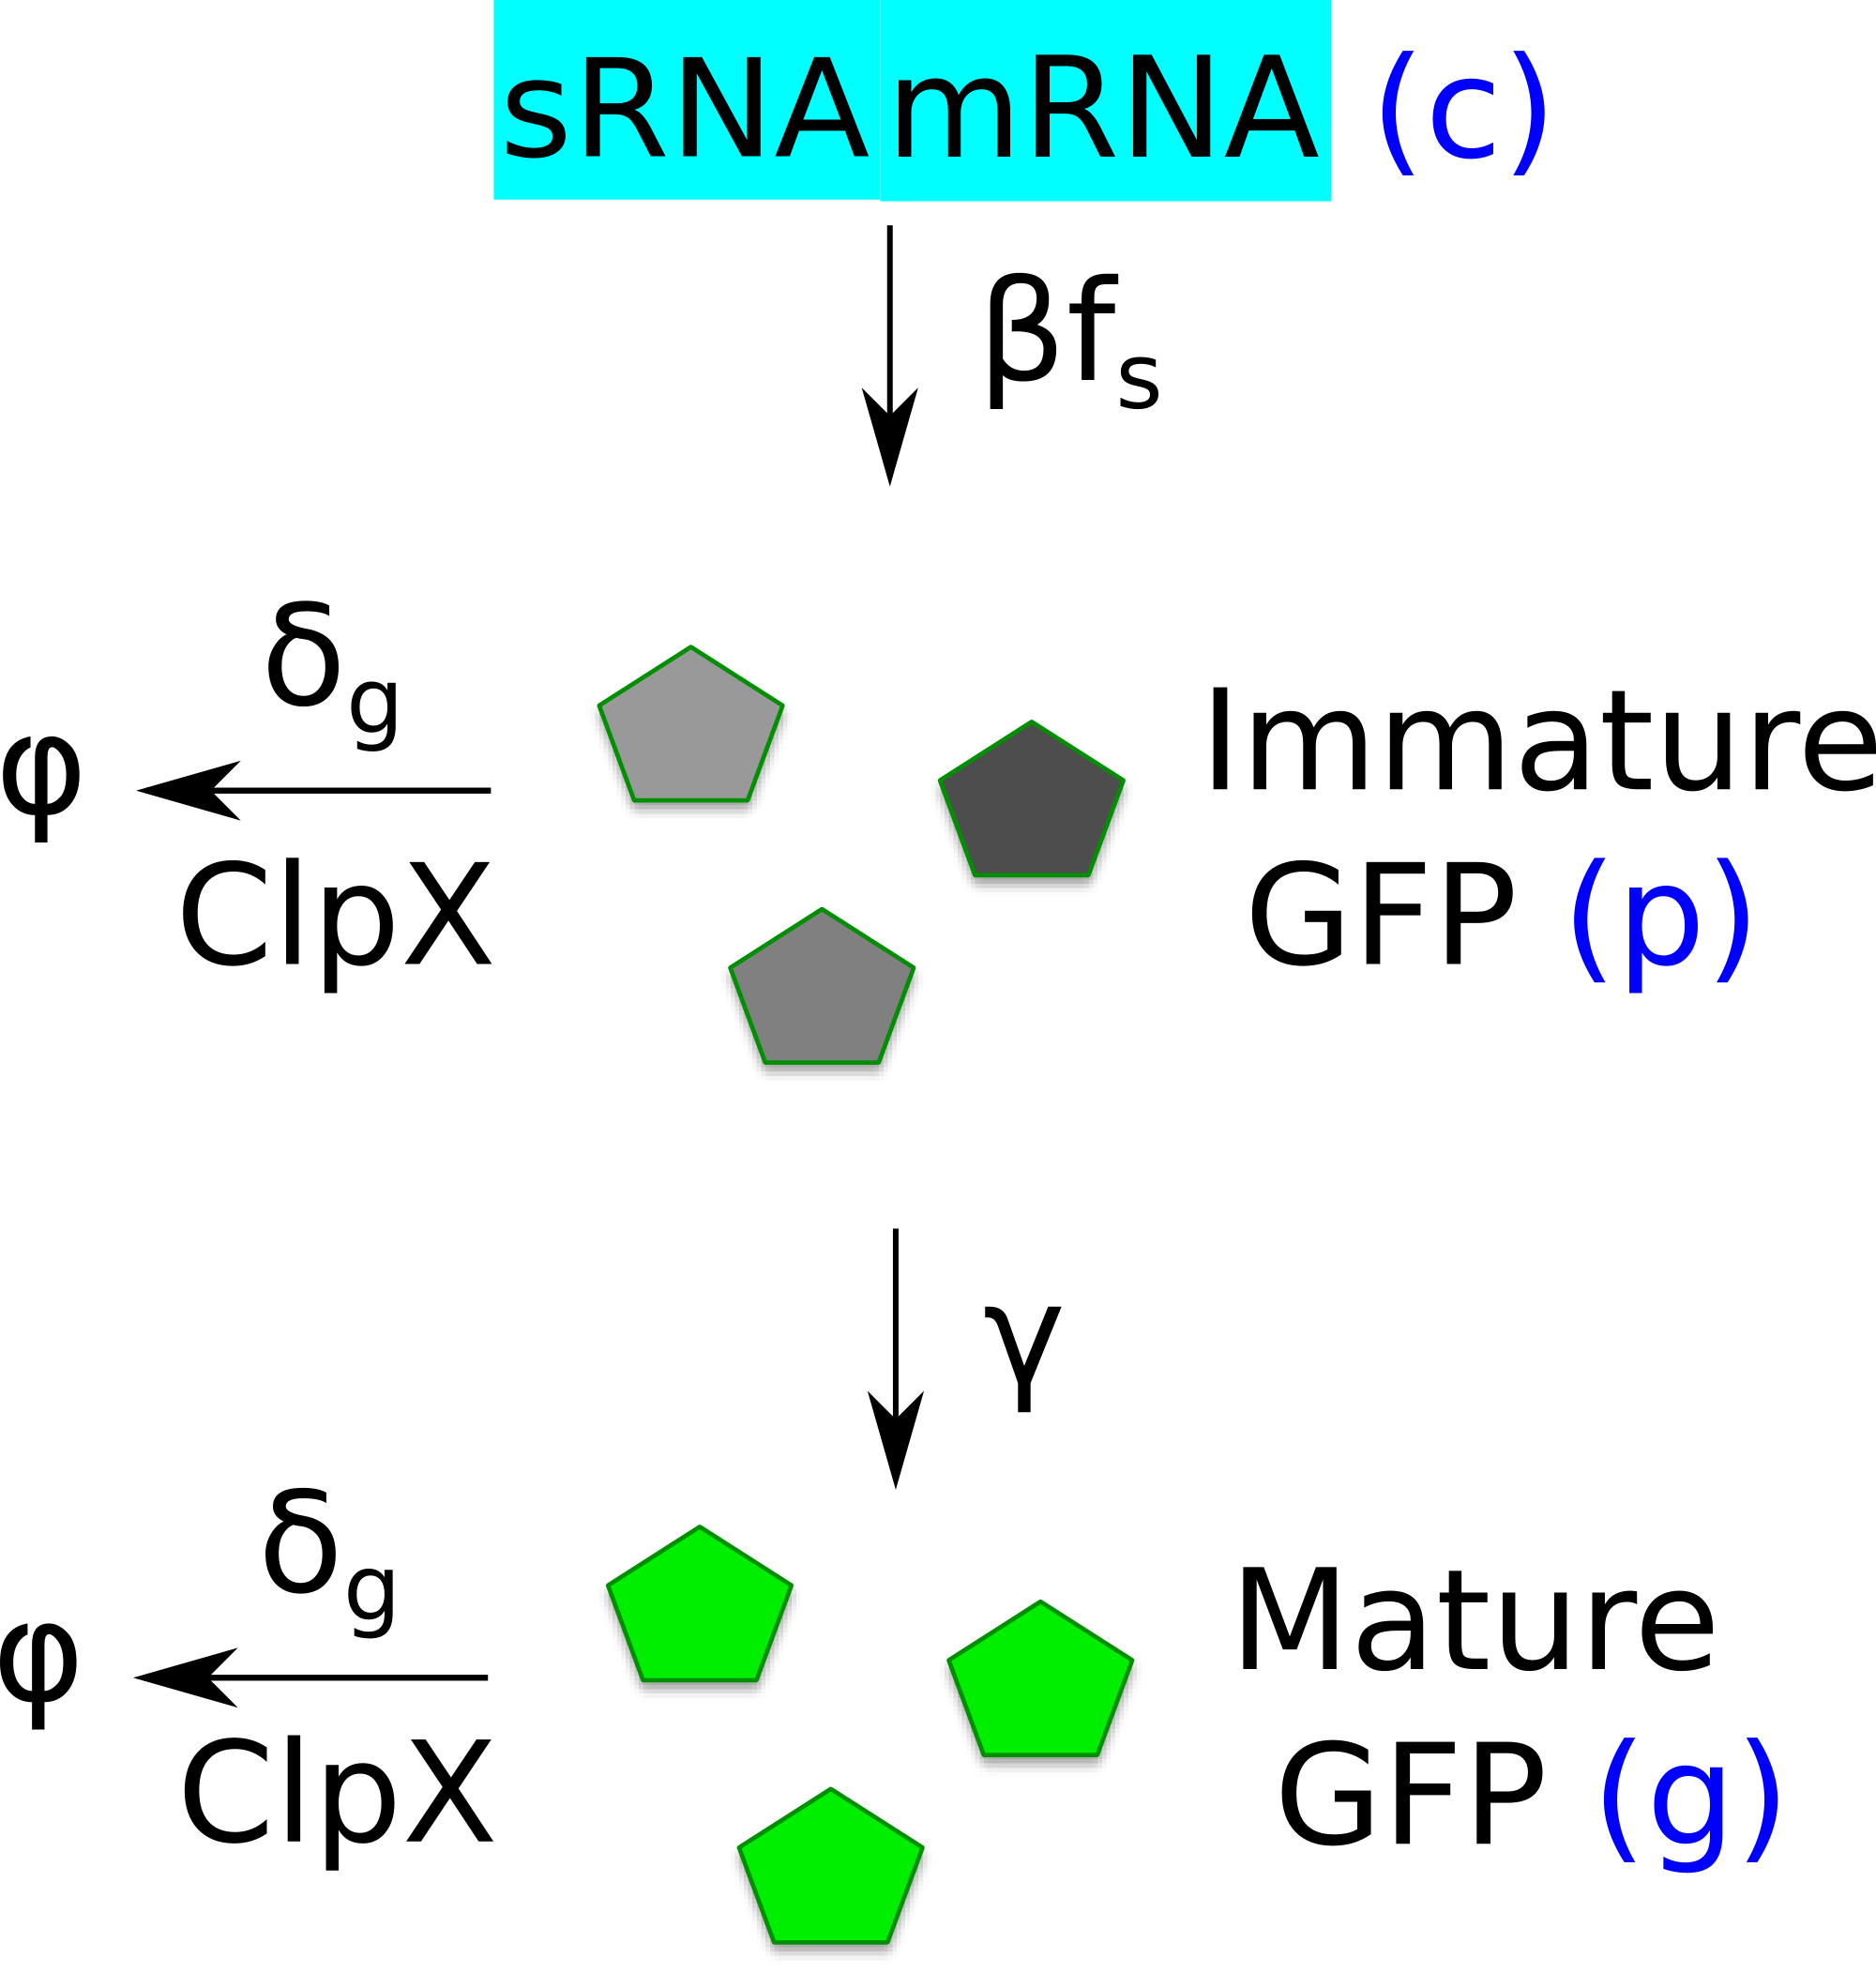
\includegraphics[trim = 0 0 0 0,clip = true,scale = 0.31]{Figures/schematic_translation}
\column{.6\textwidth}
  \begin{itemize}
    \item Translation of stable complex \textcolor{blue}{($c$)} into immature GFP \textcolor{blue}{($p$)}. 
    \item maturation of GFP \textcolor{blue}{($g$)}, machine calibration giving measured fluorescence \textcolor{blue}{($z$)}.
    \end{itemize}
\footnotesize
\begin{align*} 
\frac{d\textcolor{blue}{p}}{dt} & = \beta m +f_{s}\beta c -(\gamma + \mu + \delta_{g})p - \frac{v_{z}p}{K_{z}+p+g}   \\
\frac{d\textcolor{blue}{g}}{dt} & = \gamma p - (\mu + \delta_{g})g - \frac{v_{z}g}{K_{z}+p+g} \\
z &= z_{0} +\frac{g}{\Theta} 
\end{align*}
\end{columns}
\end{frame}

\section{Parameter Estimation in ODE Model}

\small
\begin{frame}{Full model, with parameters to be estimated}
\begin{align} 
\frac{ds}{dt} &= \frac{N\alpha_{T}}{f_{T}} y(t)-(\alert{\mu} + \alert{\delta_{s}})s -\alert{k_{\mathrm{on}}}sm +\alert{k_{\mathrm{off}}}s:m \\
\frac{dm}{dt} &=  \frac{N\alpha_{L}}{f_{L}}x(t)-(\alert{\mu} + \alert{\delta_{m}})m -\alert{k_{\mathrm{on}}}sm +\alert{k_{\mathrm{off}}}s:m  \\
\frac{ds:m}{dt} & = \alert{k_{\mathrm{on}}}sm  - (\alert{k_{\mathrm{off}}}+ \alert{k_{\mathrm{hyb}}})s:m  -(\alert{\mu} + \alert{\delta_{m}} )s:m \\
\frac{dc}{dt} & = \alert{k_{\mathrm{hyb}}}s:m  -(\alert{\mu} + \alert{\delta_{m}})c  
\end{align}
\begin{center}
\rule{0.5\textwidth}{.4pt}
\end{center}
\begin{align}
\frac{dp}{dt} & = \alert{\beta} m +\alert{f_{s}}\beta c -(\gamma + \alert{\mu} + \delta_{g})p - \frac{v_{z}p}{K_{z}+p+g}   \\
\frac{dg}{dt} & = \gamma p - (\alert{\mu} + \delta_{g})g - \frac{v_{z}g}{K_{z}+p+g} \\
z &= z_{0} +\frac{g}{\alert{\Theta}} 
\end{align}
\end{frame}
\normalsize

\begin{frame}{Recent experimental data}{}
   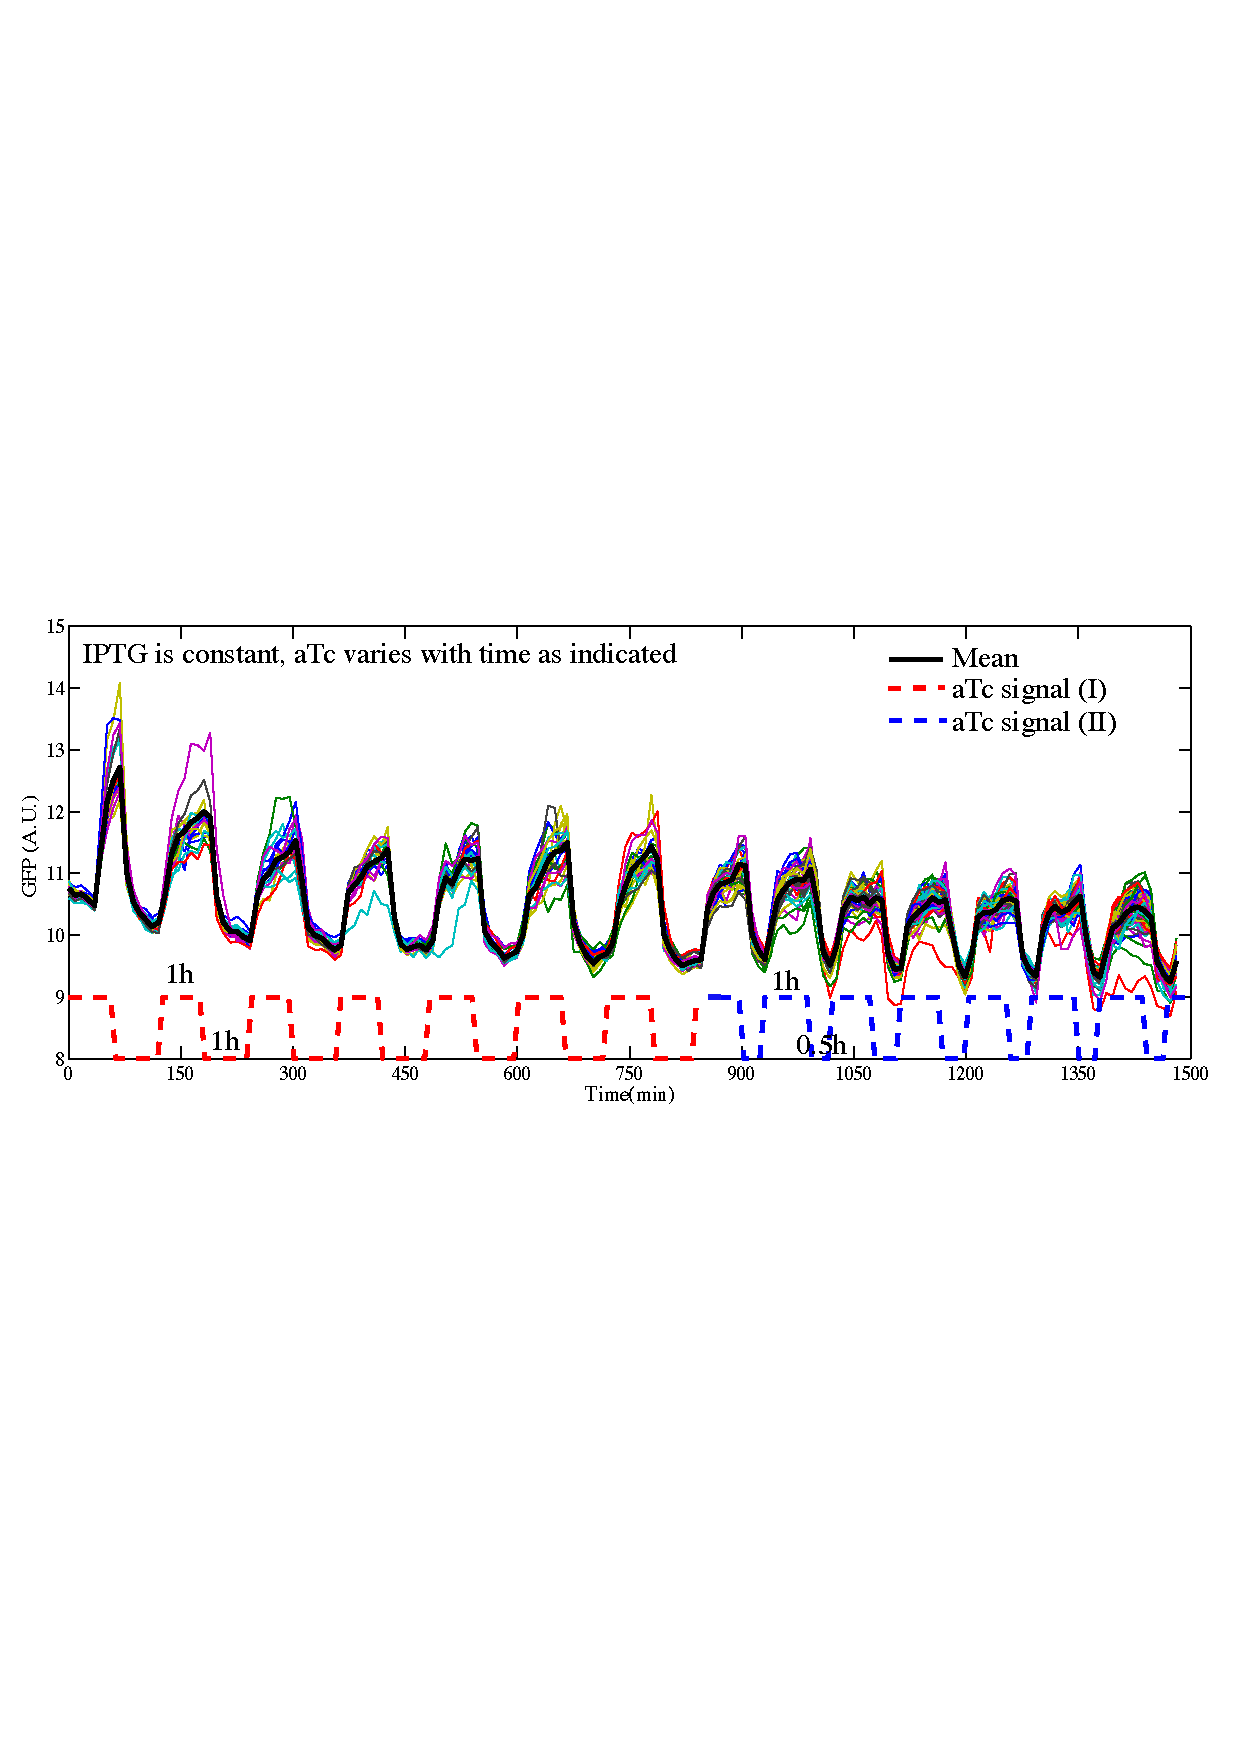
\includegraphics[trim = 0 300 0 300,clip = true,scale = 0.55]{Figures/13_9}
  \begin{itemize}
      \item  Data records $z= z_{0} +\frac{g}{\alert{\Theta}} $
    \item Single cell fluoresence time series data (Jaramillo Lab, unpublished).
    \end{itemize}
\end{frame}


\subsection{Methodology - least squares error minimisation}

\begin{frame}{Method for parameter estimation in ODE model}
  \begin{block}{Goal}
 Estimate unknown parameters in model using time series data.
    \end{block}
    
      \begin{itemize}
    \item  Least squares error minimization approach
    \begin{align*}
\argmin_{\boldsymbol{\theta}} \sum_{i =1}^{n} (z_{\mathrm{exp, mean}}(t_{i}) - z(t_{i},\boldsymbol{\theta}))^2.
\end{align*}
\item Used evolutionary algorithm to perform minimisation.
    \end{itemize}
\end{frame}

\subsection{Results - Inestimable parameters, model simplifications}

\begin{frame}{Initial estimation results}
  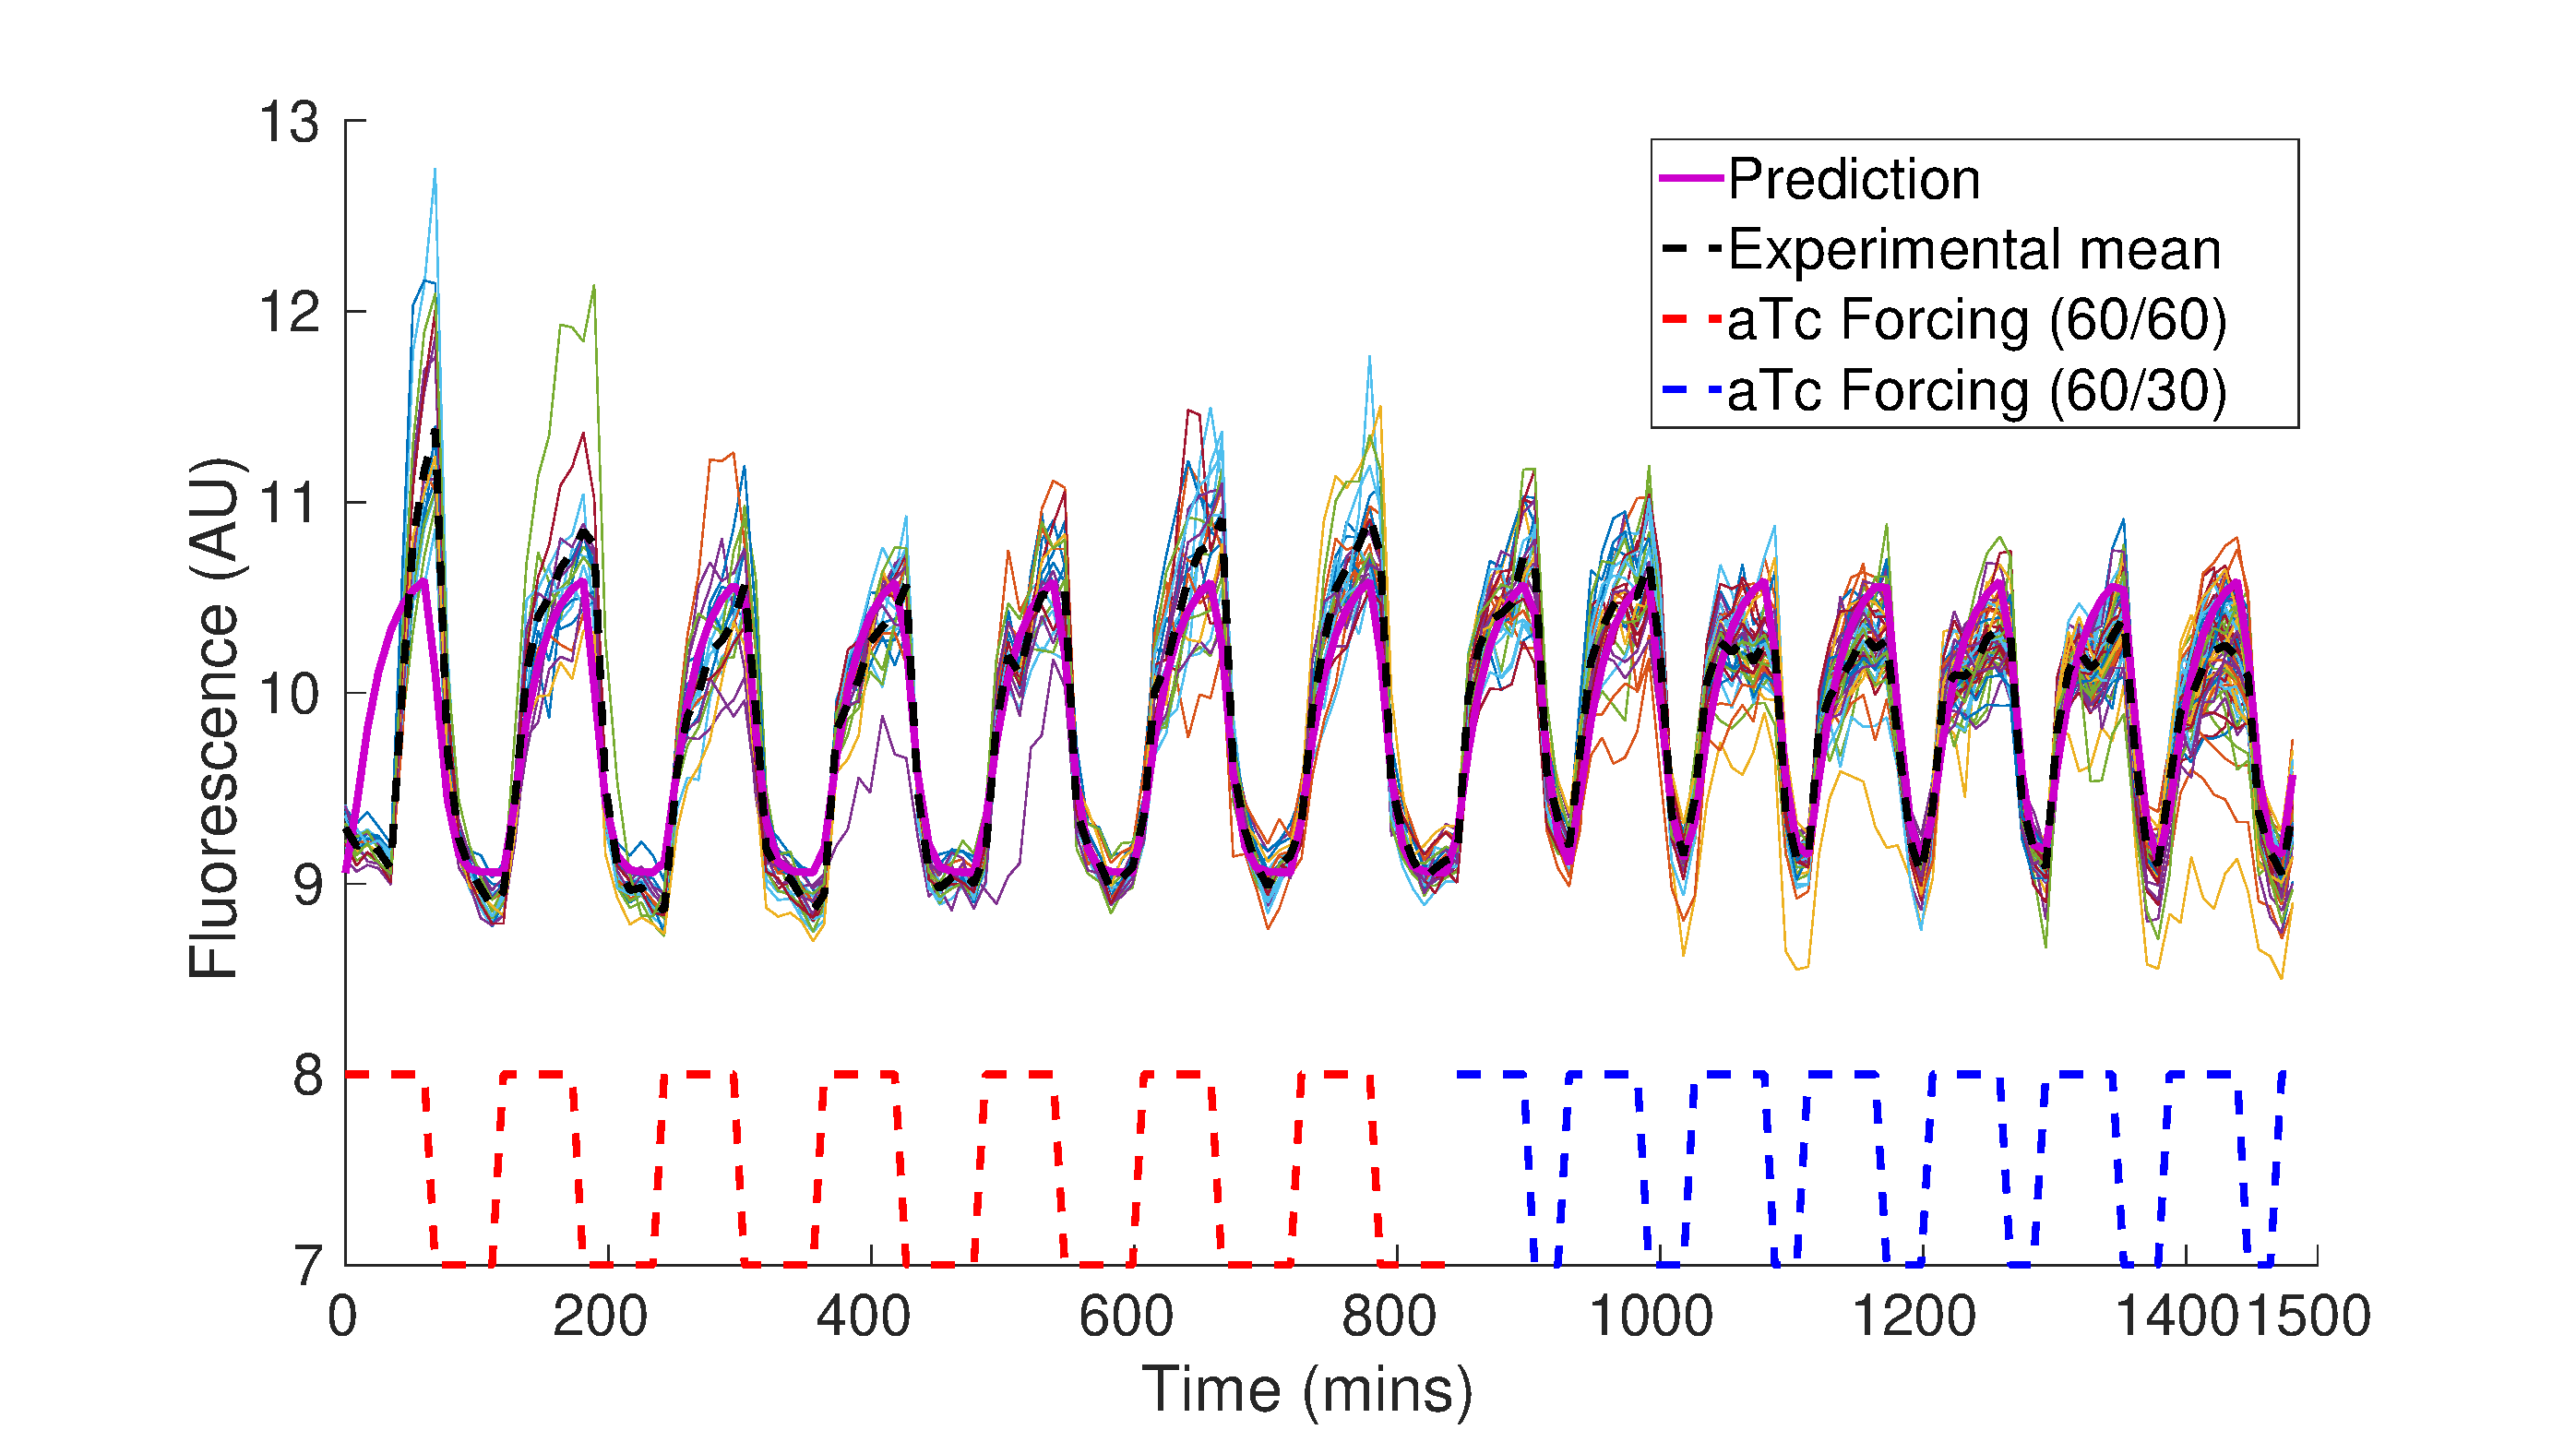
\includegraphics[scale = 0.28, clip = true, trim = 80 0 0 0]{Figures/13_9_bestPlot}
\end{frame}


\begin{frame}{Initial estimation results}
  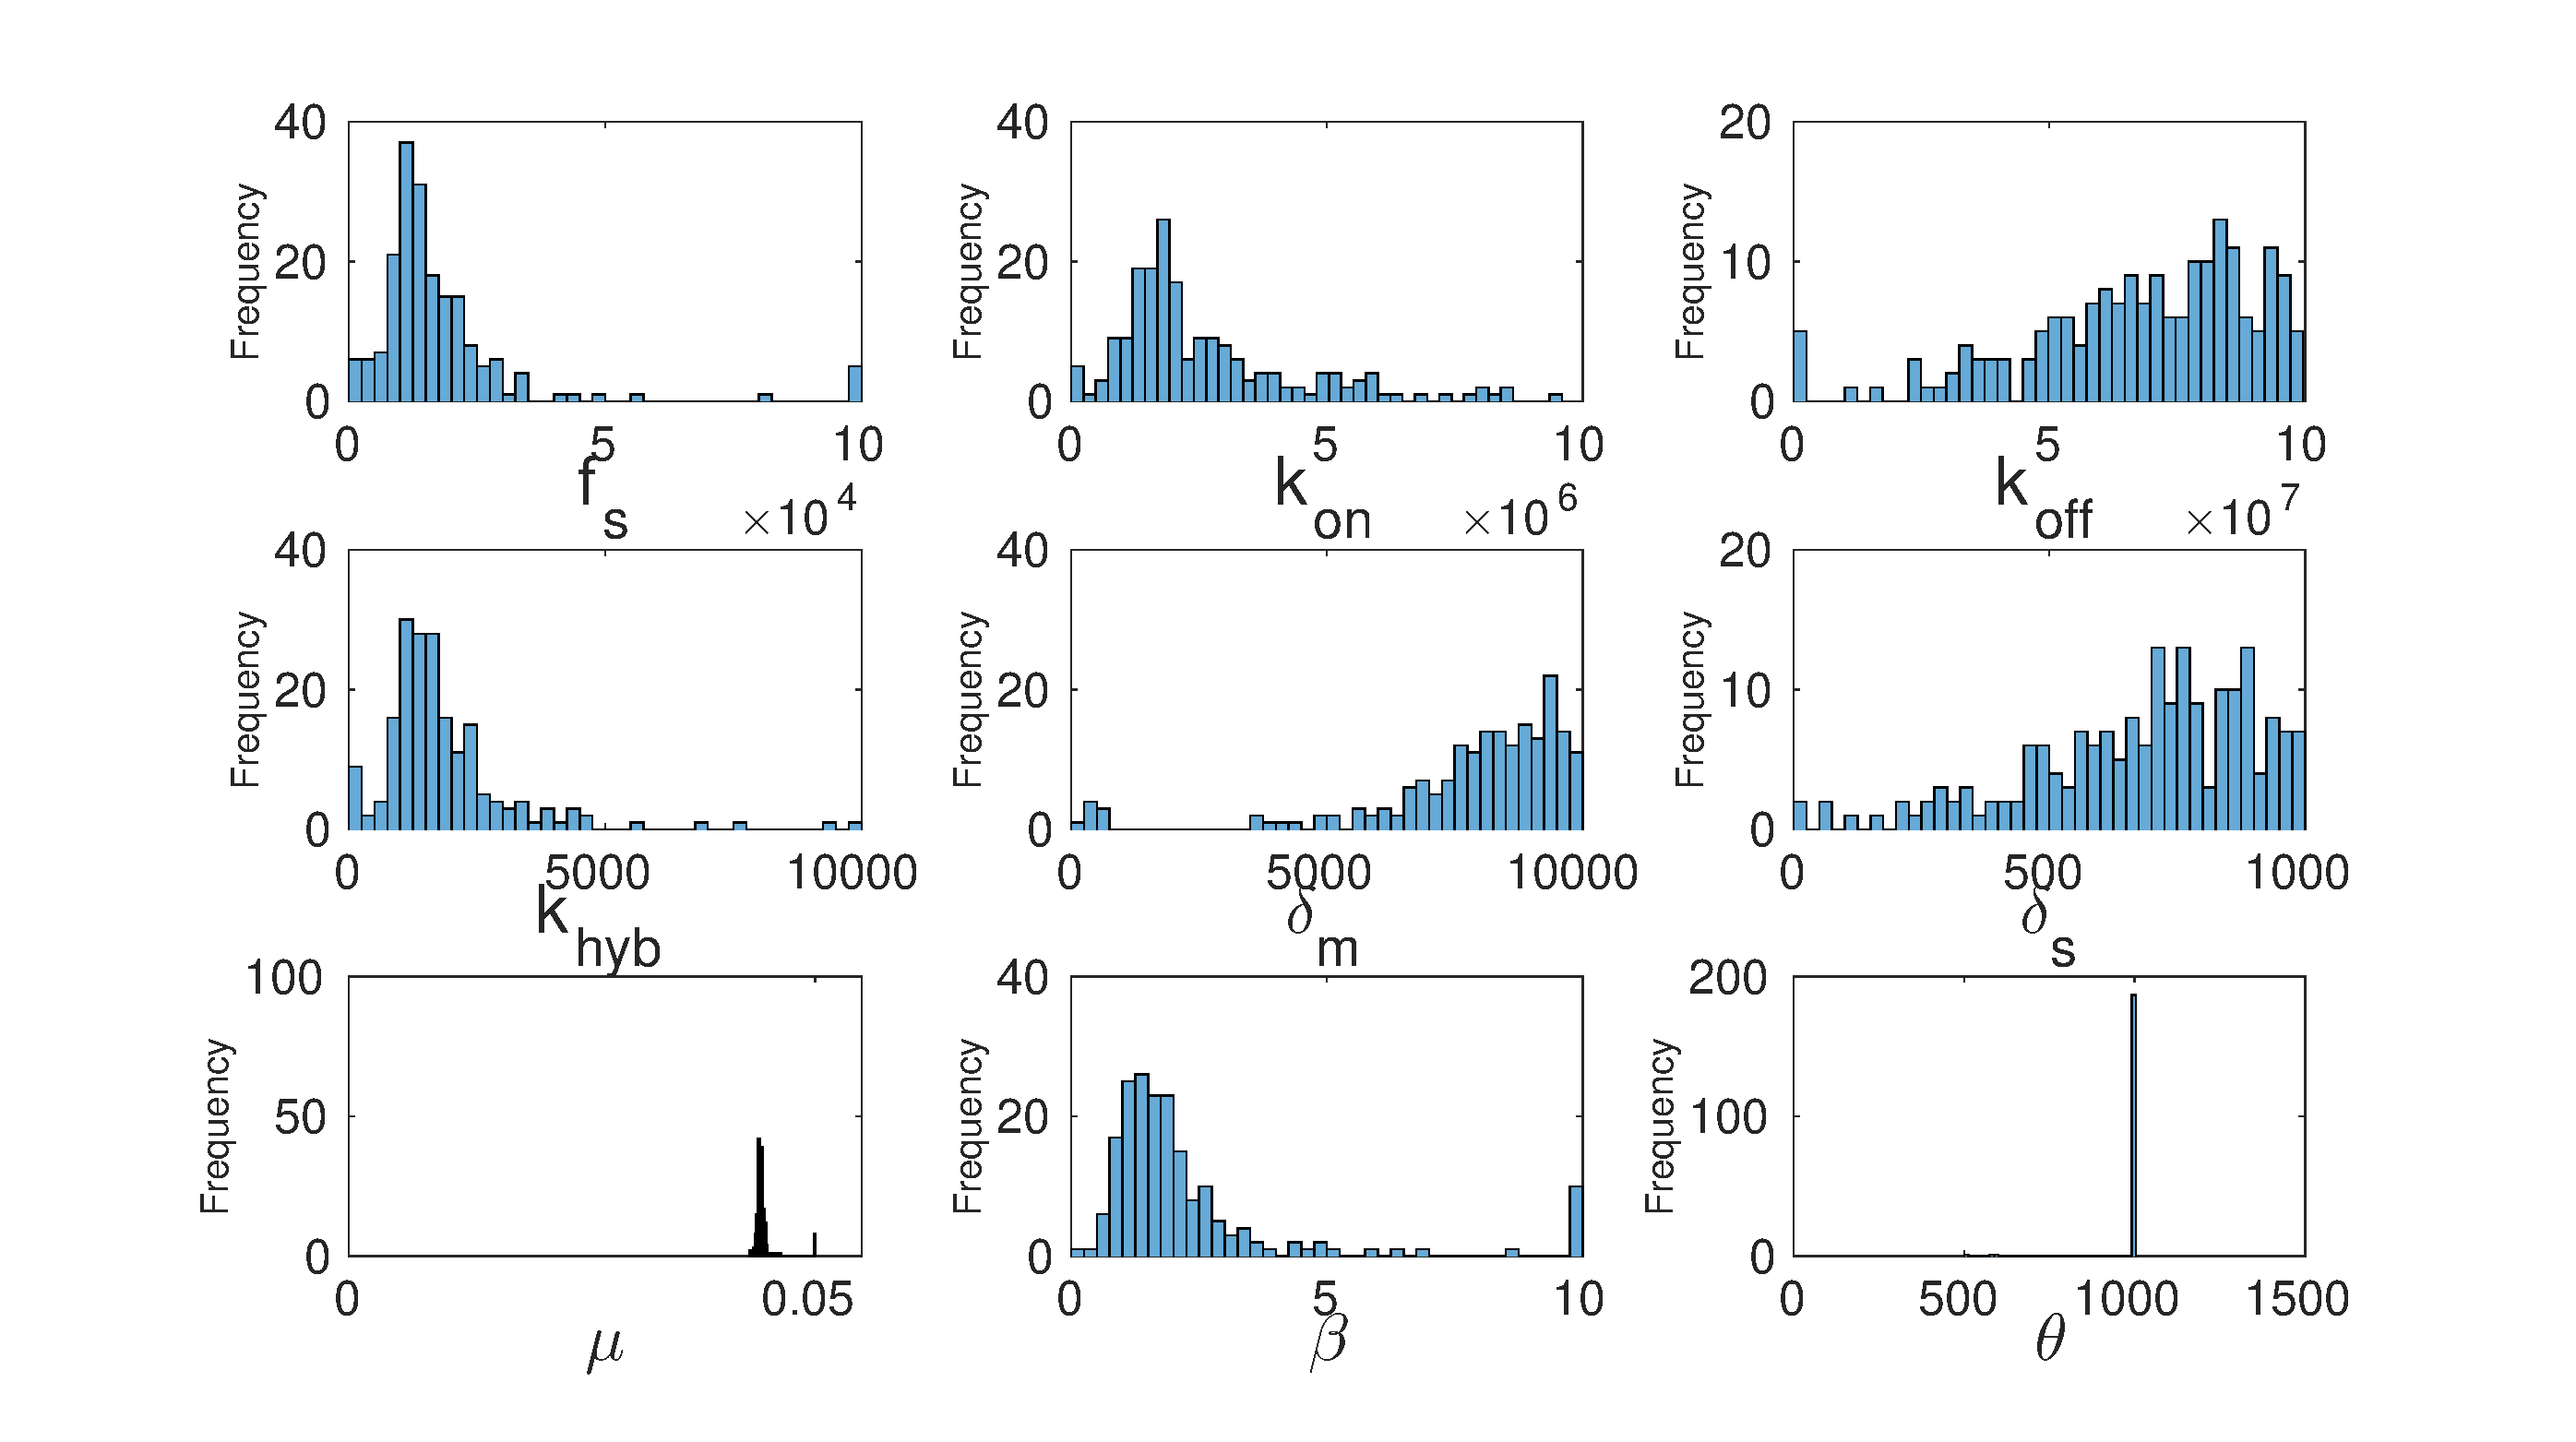
\includegraphics[scale = 0.27, clip = true, trim = 100 0 0 40]{Figures/13_9_hist}
  \vspace{-10mm}
        \begin{itemize}
            \item Many parameters poorly estimated.
    \item Similar error values for all results.
            \end{itemize}
\end{frame}

\begin{frame}{Sensitivity analysis}
\begin{columns}
\column{.4\textwidth}
 \LARGE
\begin{align*}
S_{ij} =  \frac{\partial z}{ \partial \theta_{j}}\Bigr|_{t_{i}}
\end{align*}
\normalsize
\column{.59\textwidth}
Perturbations of parameters all give similar effects on model output - \alert{hard to distinguish}
\end{columns}
  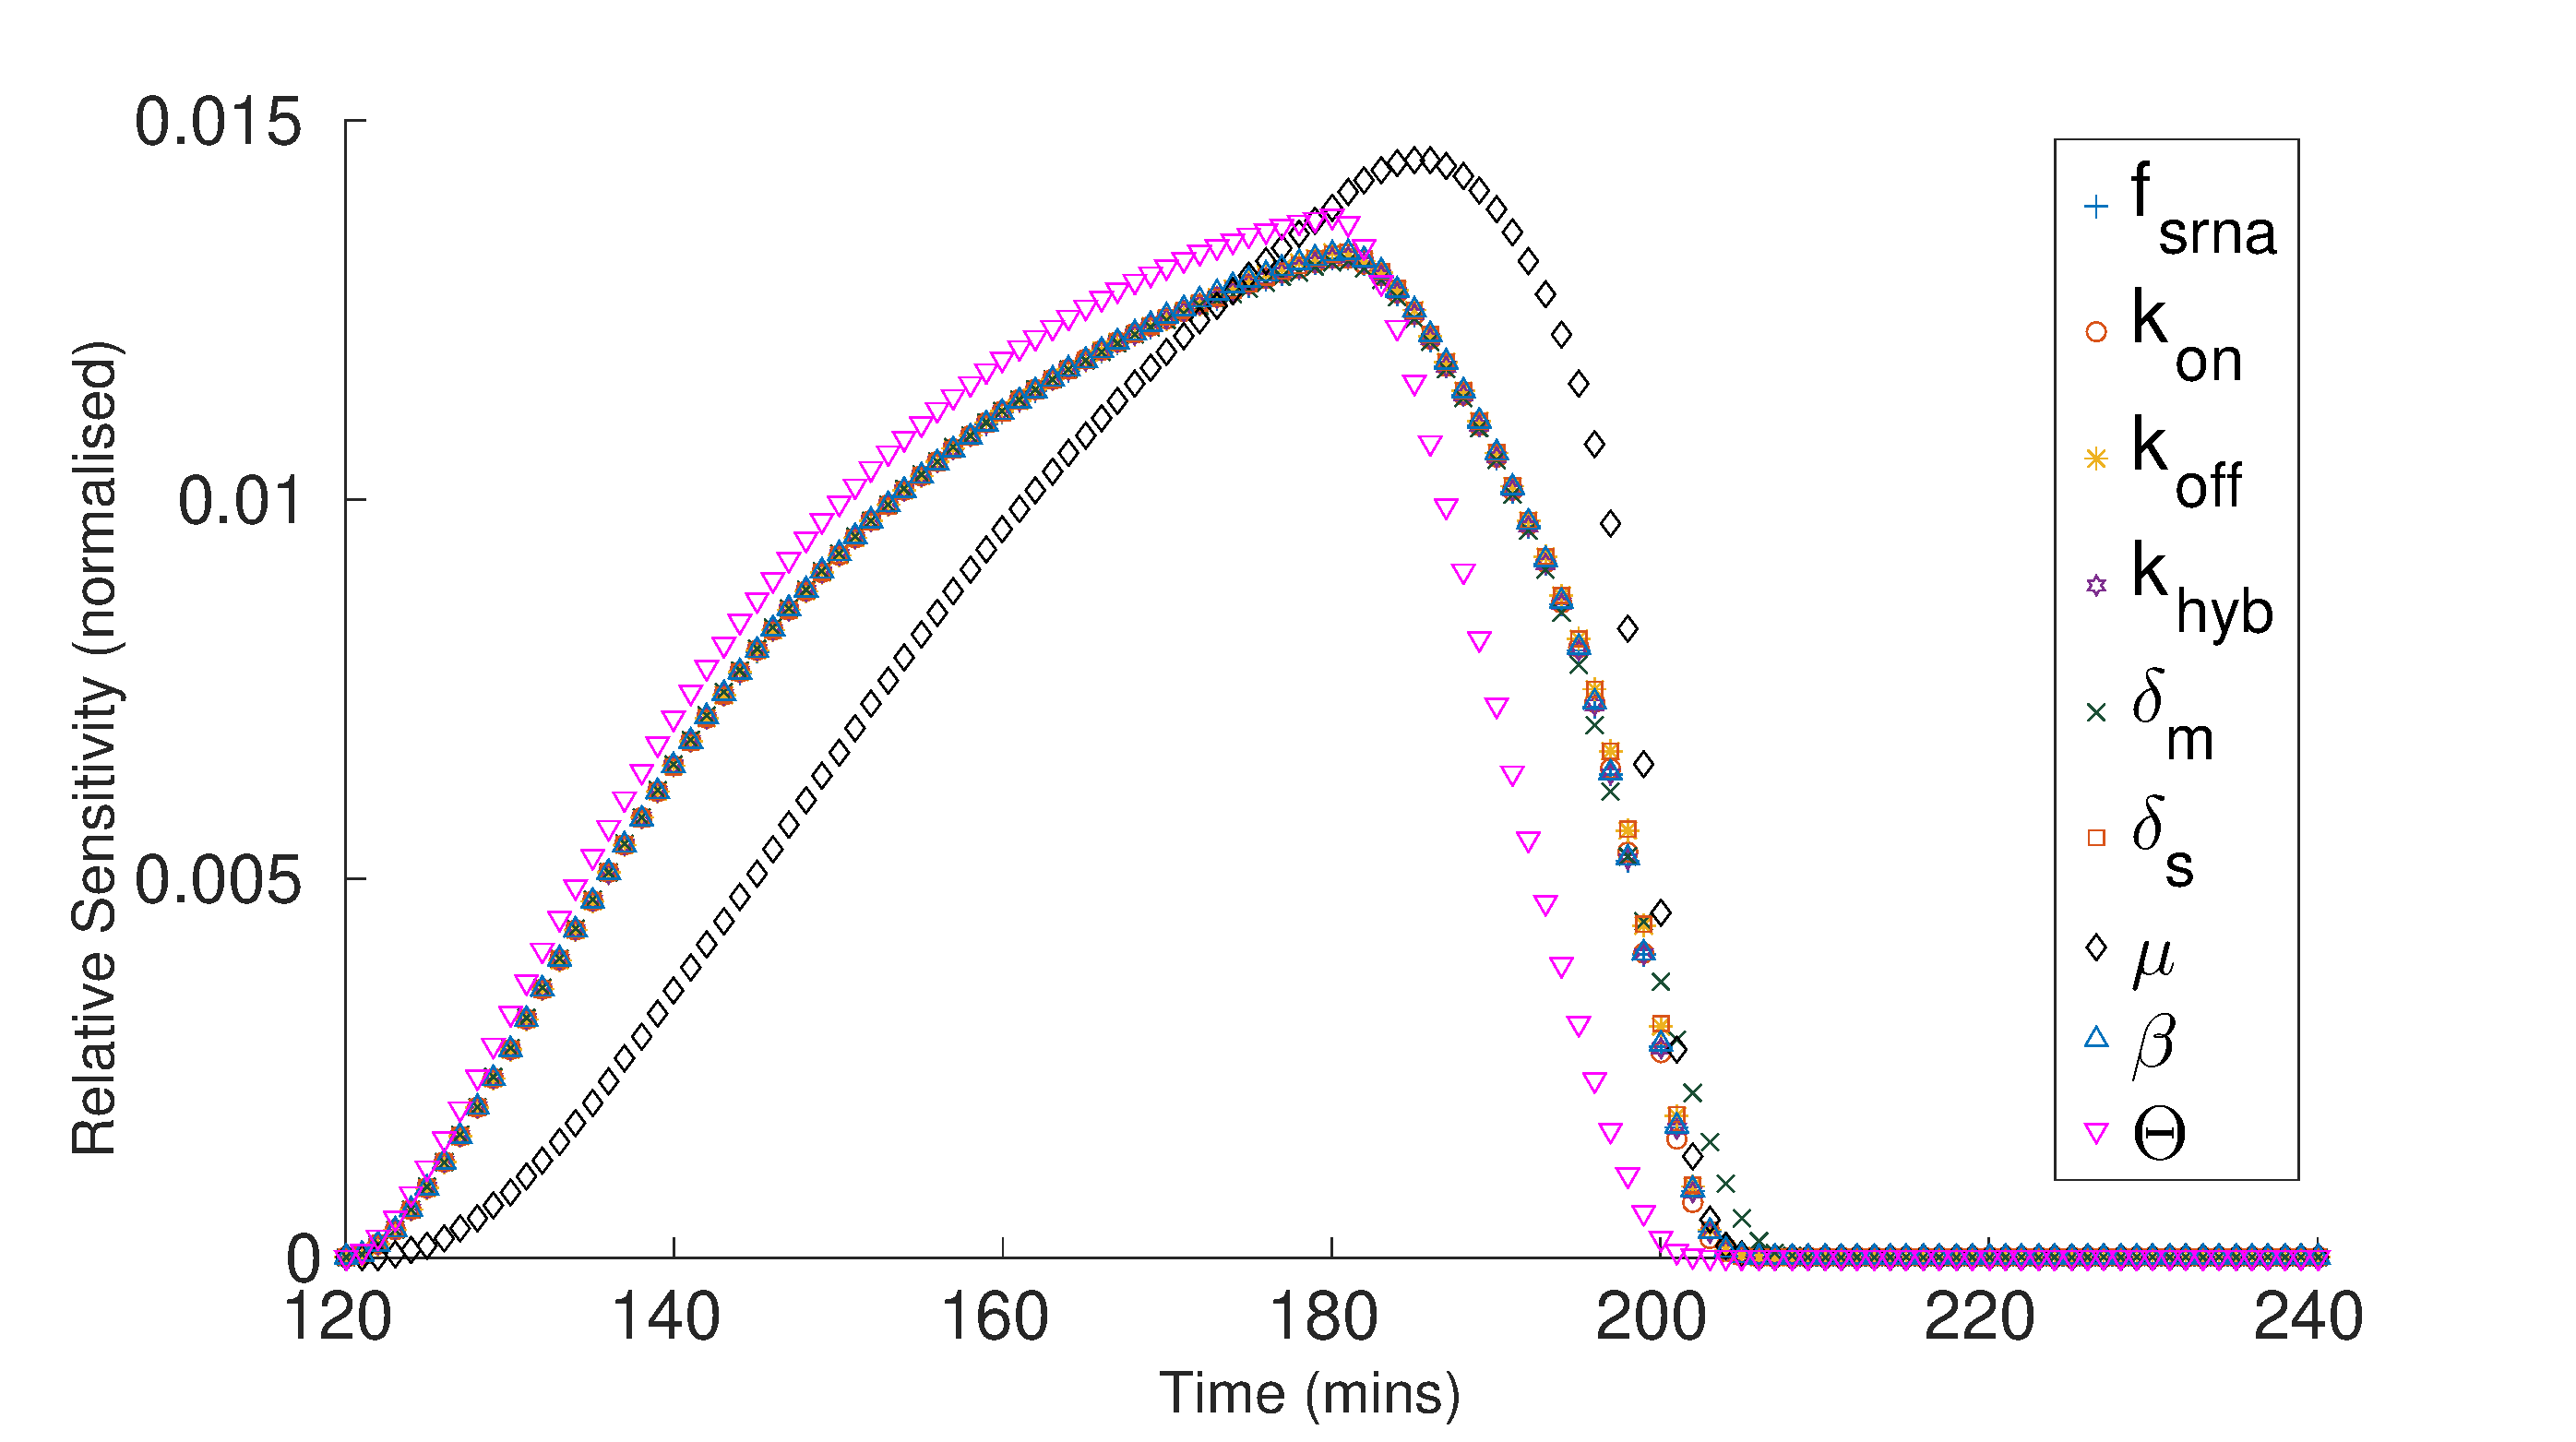
\includegraphics[scale = 0.25, clip = true, trim = 00 0 0 0]{Figures/Sensitivty_scaled_other}
\end{frame}


\small
\begin{frame}{Plotting all states of model output}
\begin{align*} 
\frac{ds}{dt} &= \frac{N\alpha_{T}}{f_{T}} y(t)-(\alert{\mu} + \alert{\delta_{s}})s -\alert{k_{\mathrm{on}}}sm +\alert{k_{\mathrm{off}}}s:m \\
\frac{dm}{dt} &=  \frac{N\alpha_{L}}{f_{L}}x(t)-(\alert{\mu} + \alert{\delta_{m}})m -\alert{k_{\mathrm{on}}}sm +\alert{k_{\mathrm{off}}}s:m  \\
\frac{ds:m}{dt} & = \alert{k_{\mathrm{on}}}sm  - (\alert{k_{\mathrm{off}}}+ \alert{k_{\mathrm{hyb}}})s:m  -(\alert{\mu} + \alert{\delta_{m}} )s:m \\
\frac{dc}{dt} & = \alert{k_{\mathrm{hyb}}}s:m  -(\alert{\mu} + \alert{\delta_{m}})c  
\end{align*}
\begin{center}
\rule{0.5\textwidth}{.4pt}
\end{center}
\begin{align*}
\frac{dp}{dt} & = \alert{\beta} m +\alert{f_{s}}\beta c -(\gamma + \alert{\mu} + \delta_{g})p - \frac{v_{z}p}{K_{z}+p+g}   \\
\frac{dg}{dt} & = \gamma p - (\alert{\mu} + \delta_{g})g - \frac{v_{z}g}{K_{z}+p+g} \\
z &= z_{0} +\frac{g}{\alert{\Theta}} 
\end{align*}
\end{frame}
\normalsize


\begin{frame}{Model output for all state variables}
  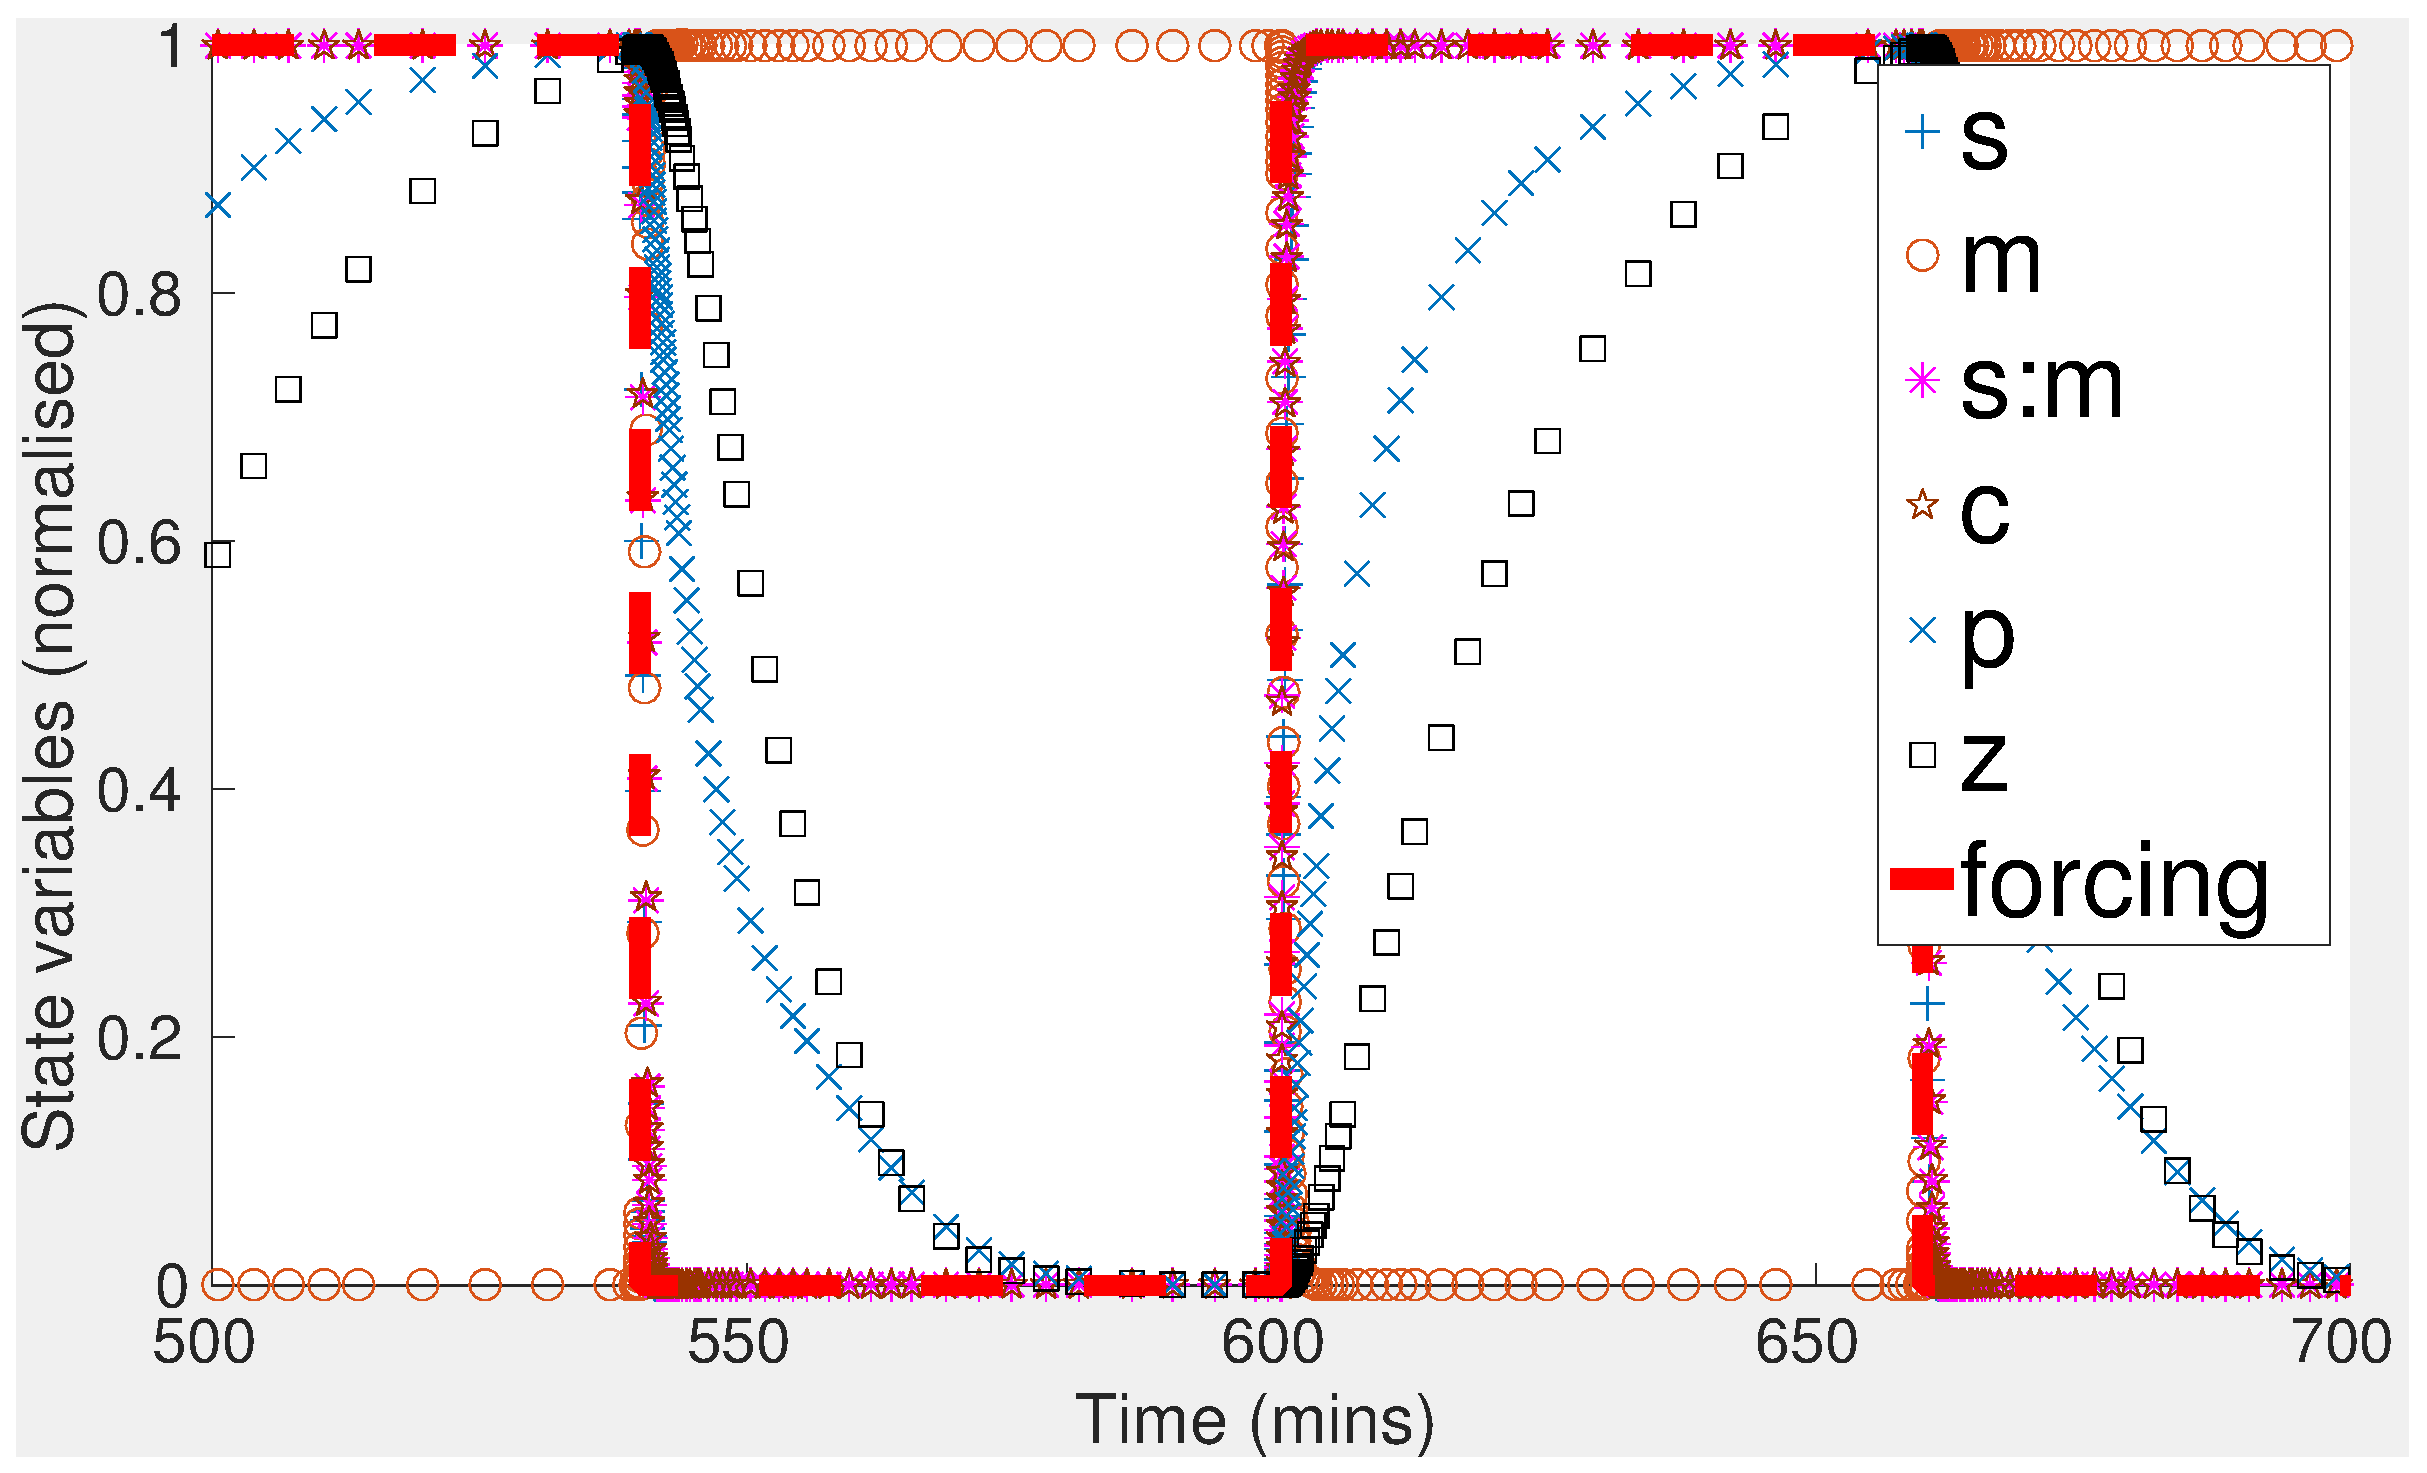
\includegraphics[scale = 0.26, clip = true, trim = 0 0 0 0]{Figures/model_output}
  \begin{itemize}
    \item $s,m,s:m,c$ \alert{(binding step)} respond instantly to forcing.
    \item $p, z$ \alert{(translation step)} on timescale of forcing.
\end{itemize}
\end{frame}

\footnotesize
\begin{frame}{Translation rate limiting}
\begin{align*} 
\frac{ds}{dt} &= \frac{N\alpha_{T}}{f_{T}} y(t)-(\alert{\mu} + \alert{\delta_{s}})s -\alert{k_{\mathrm{on}}}sm +\alert{k_{\mathrm{off}}}s:m \\
\frac{dm}{dt} &=  \frac{N\alpha_{L}}{f_{L}}x(t)-(\alert{\mu} + \alert{\delta_{m}})m -\alert{k_{\mathrm{on}}}sm +\alert{k_{\mathrm{off}}}s:m  \\
\frac{ds:m}{dt} & = \alert{k_{\mathrm{on}}}sm  - (\alert{k_{\mathrm{off}}}+ \alert{k_{\mathrm{hyb}}})s:m  -(\alert{\mu} + \alert{\delta_{m}} )s:m \\
\frac{dc}{dt} & = \alert{k_{\mathrm{hyb}}}s:m  -(\alert{\mu} + \alert{\delta_{m}})c  
\end{align*}
\begin{center}
\rule{0.5\textwidth}{.4pt}
\end{center}
\begin{align*} 
\frac{dp}{dt} & = \alert{\beta} m +\alert{f_{s}}\beta c -(\gamma + \alert{\mu} + \delta_{g})p - \frac{v_{z}p}{K_{z}+p+g}   \\
\frac{dg}{dt} & = \gamma p - (\alert{\mu} + \delta_{g})g - \frac{v_{z}g}{K_{z}+p+g} \\
z &= z_{0} +\frac{g}{\alert{\Theta}} 
\end{align*}
\normalsize
\vspace{-5mm}
  \begin{itemize}
  \item Binding equations respond instantly.
    \item $ \alert{\beta} m +\alert{f_{s}}\beta c $ term links binding and translation. It flips between fixed point values.
    \item All parameters `upstream' have identical effects.
\end{itemize}
\end{frame}


\small
\begin{frame}{Simplified model}
\begin{greyedout}
\begin{align*} 
\frac{ds}{dt} &= \frac{N\alpha_{T}}{f_{T}} y(t)-(\mu + \delta_{s})s -k_{\mathrm{on}}sm +k_{\mathrm{off}}s:m \\
\frac{dm}{dt} &=  \frac{N\alpha_{L}}{f_{L}}x(t)-(\mu + \delta_{m})m -k_{\mathrm{on}}sm +k_{\mathrm{off}}s:m  \\
\frac{ds:m}{dt} & = k_{\mathrm{on}}sm  - (k_{\mathrm{off}}+ k_{\mathrm{hyb}})s:m  -(\mu + \delta_{sm} )s:m \\
\frac{dc}{dt} & = k_{\mathrm{hyb}}s:m  -(\mu + \delta_{c})c  
\end{align*}
\end{greyedout}
\begin{center}
\rule{0.5\textwidth}{.4pt}
\end{center}
\begin{align*} 
\frac{dp}{dt} & = \alert{F}y(t)-(\gamma + \alert{\mu} + \delta_{g})p - \frac{v_{z}p}{K_{z}+p+g}   \\
\frac{dg}{dt} & = \gamma p - (\alert{\mu} + \delta_{g})g - \frac{v_{z}g}{K_{z}+p+g}  \\
z &= z_{0} +\frac{g}{\alert{\Theta}}  
\end{align*}
\end{frame}
\normalsize



\begin{frame}{Simplified model}
\begin{align}
\frac{dp}{dt} & = \alert{F}y(t)-(\gamma + \alert{\mu} + \delta_{g})p - \frac{v_{z}p}{K_{z}+p+g}   \\
\frac{dg}{dt} & = \gamma p - (\mu + \delta_{g})g - \frac{v_{z}g}{K_{z}+p+g}  \\
z &= z_{0} +\frac{g}{\alert{\Theta}} 
\end{align}
\begin{itemize}
\item  Model only rate limiting steps - force translation term directly.
\item 3 unknown parameters
\end{itemize}
\end{frame}


\begin{frame}{Simplified model results (1)}
  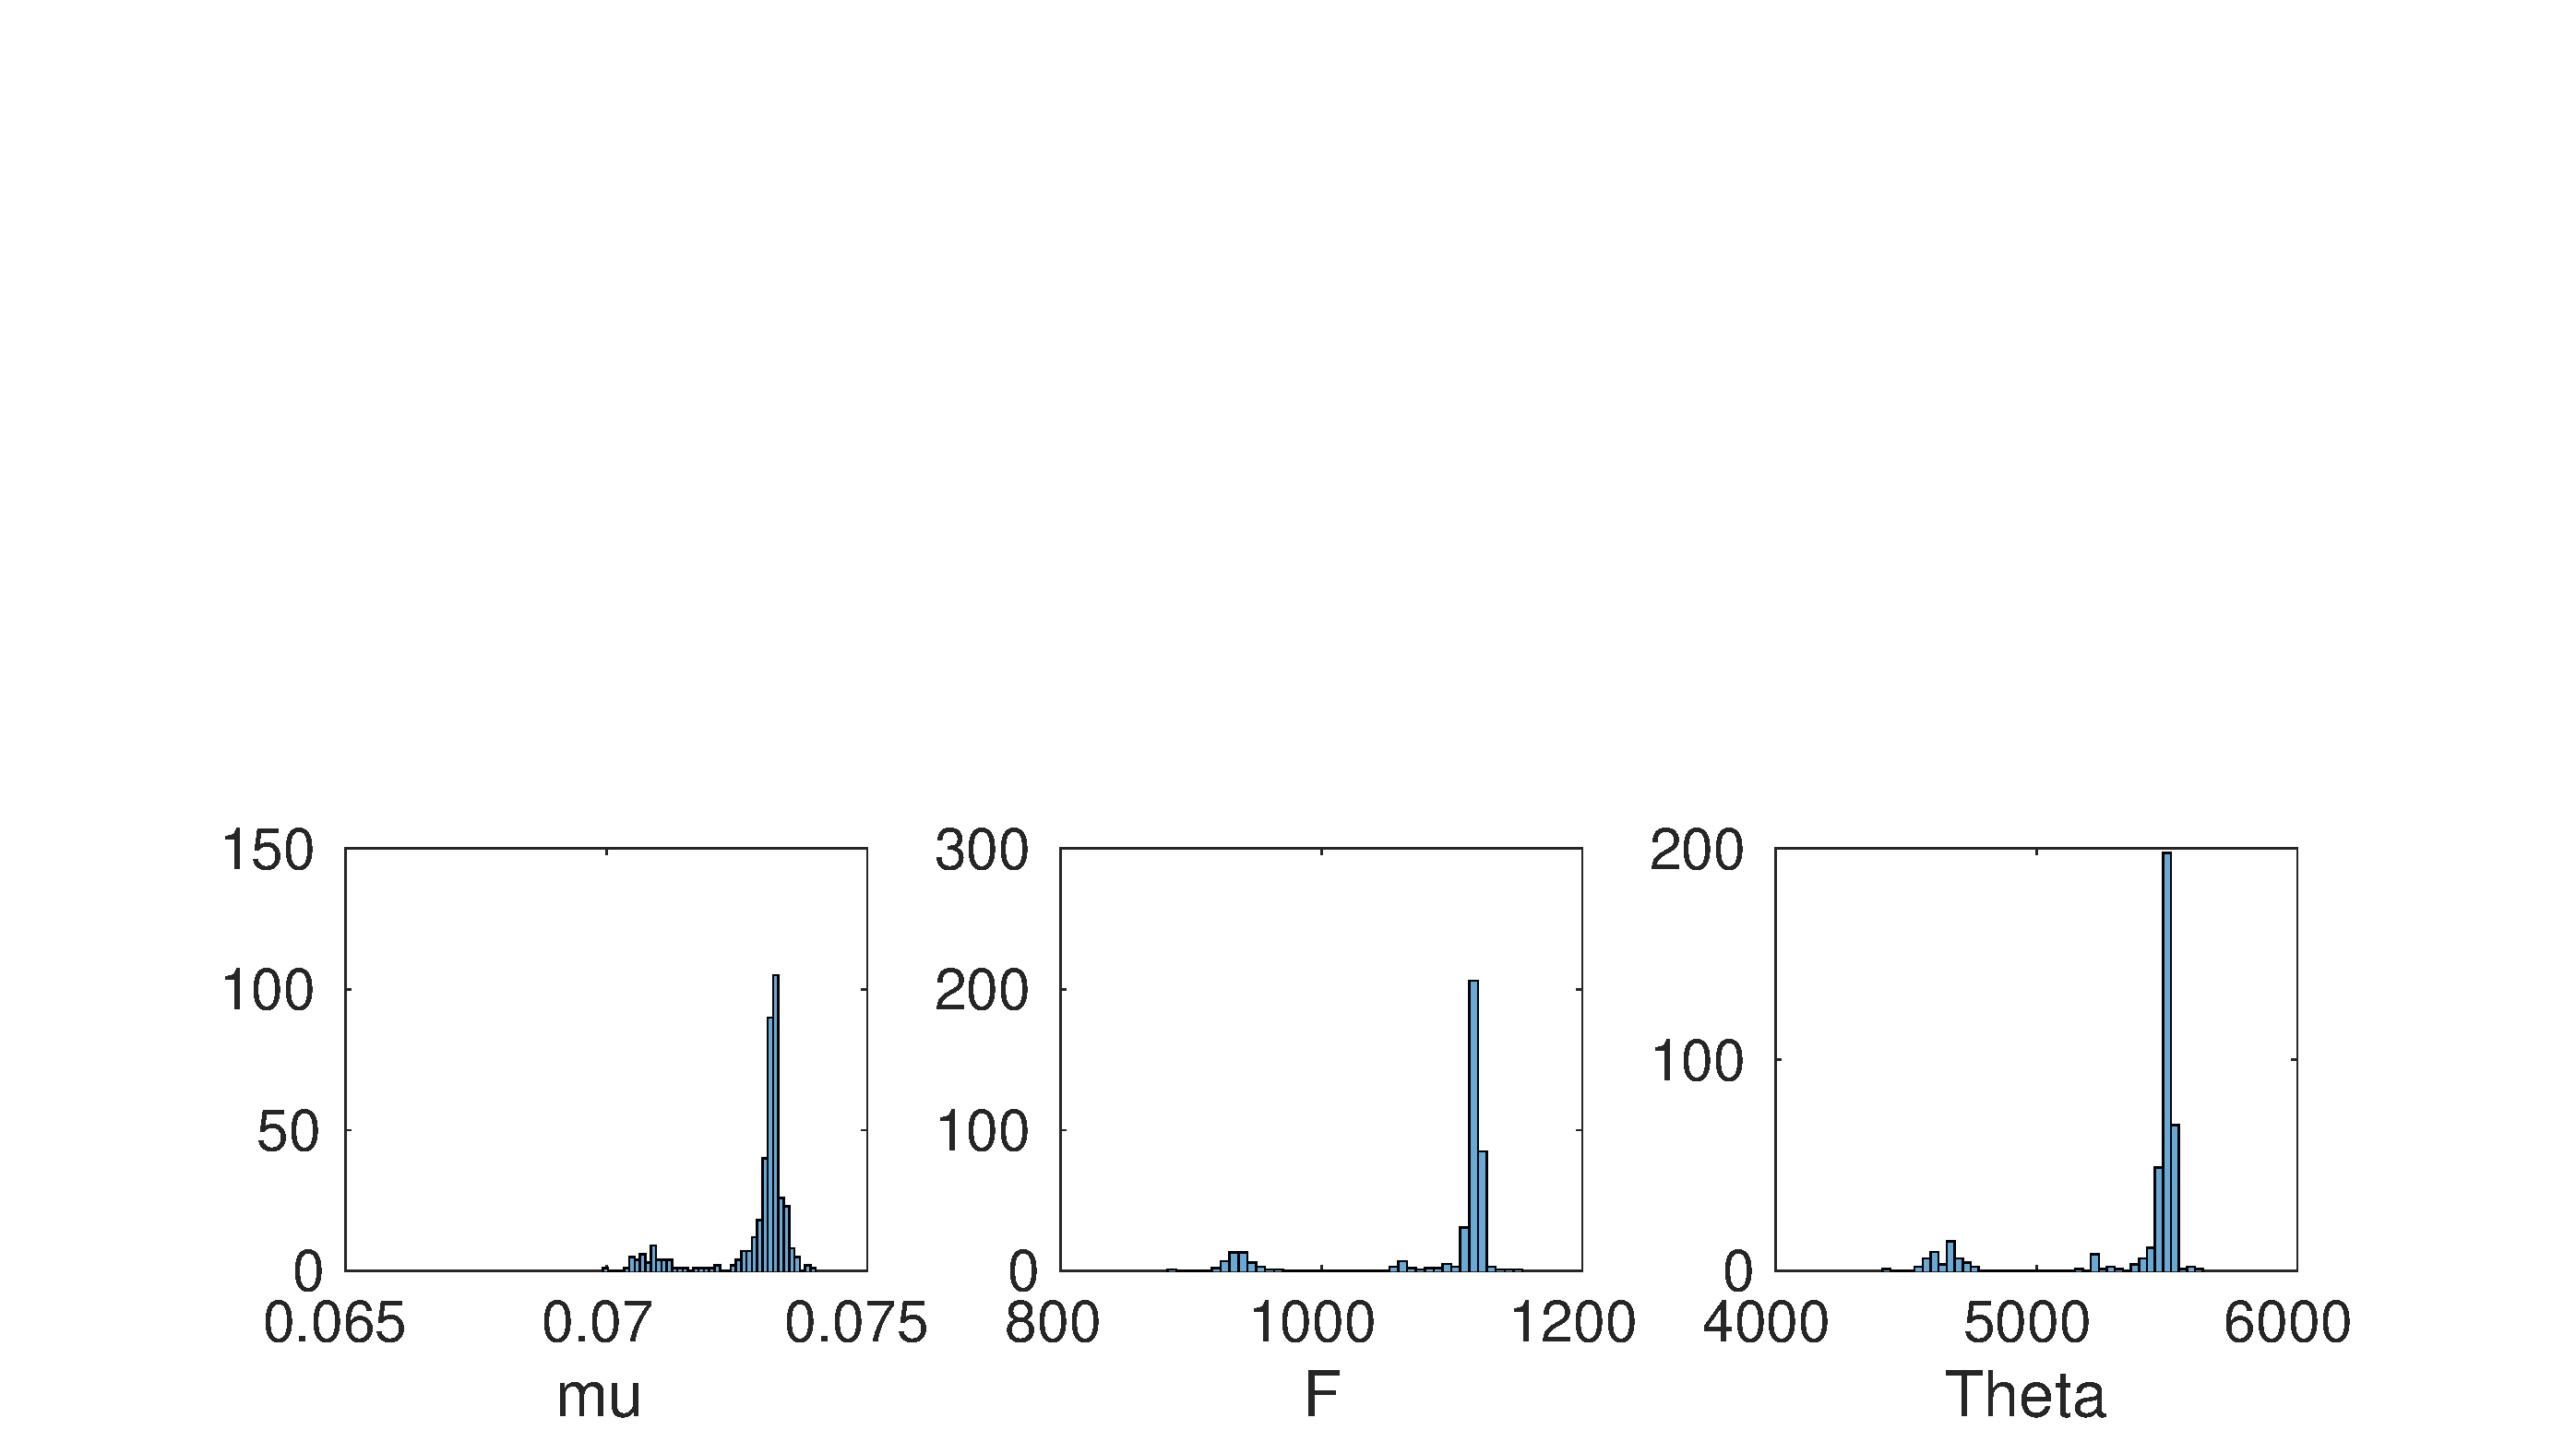
\includegraphics[scale = 0.29, clip = true, trim = 70 0 0 400]{Figures/13_9_hist_simplified}
  \begin{itemize}
\item  Error values as low as full model
\item Clearer parameter estimation results
\item Two peak structure due to local minima
\end{itemize}
\end{frame}

\begin{frame}{Simplified model results (2)}
  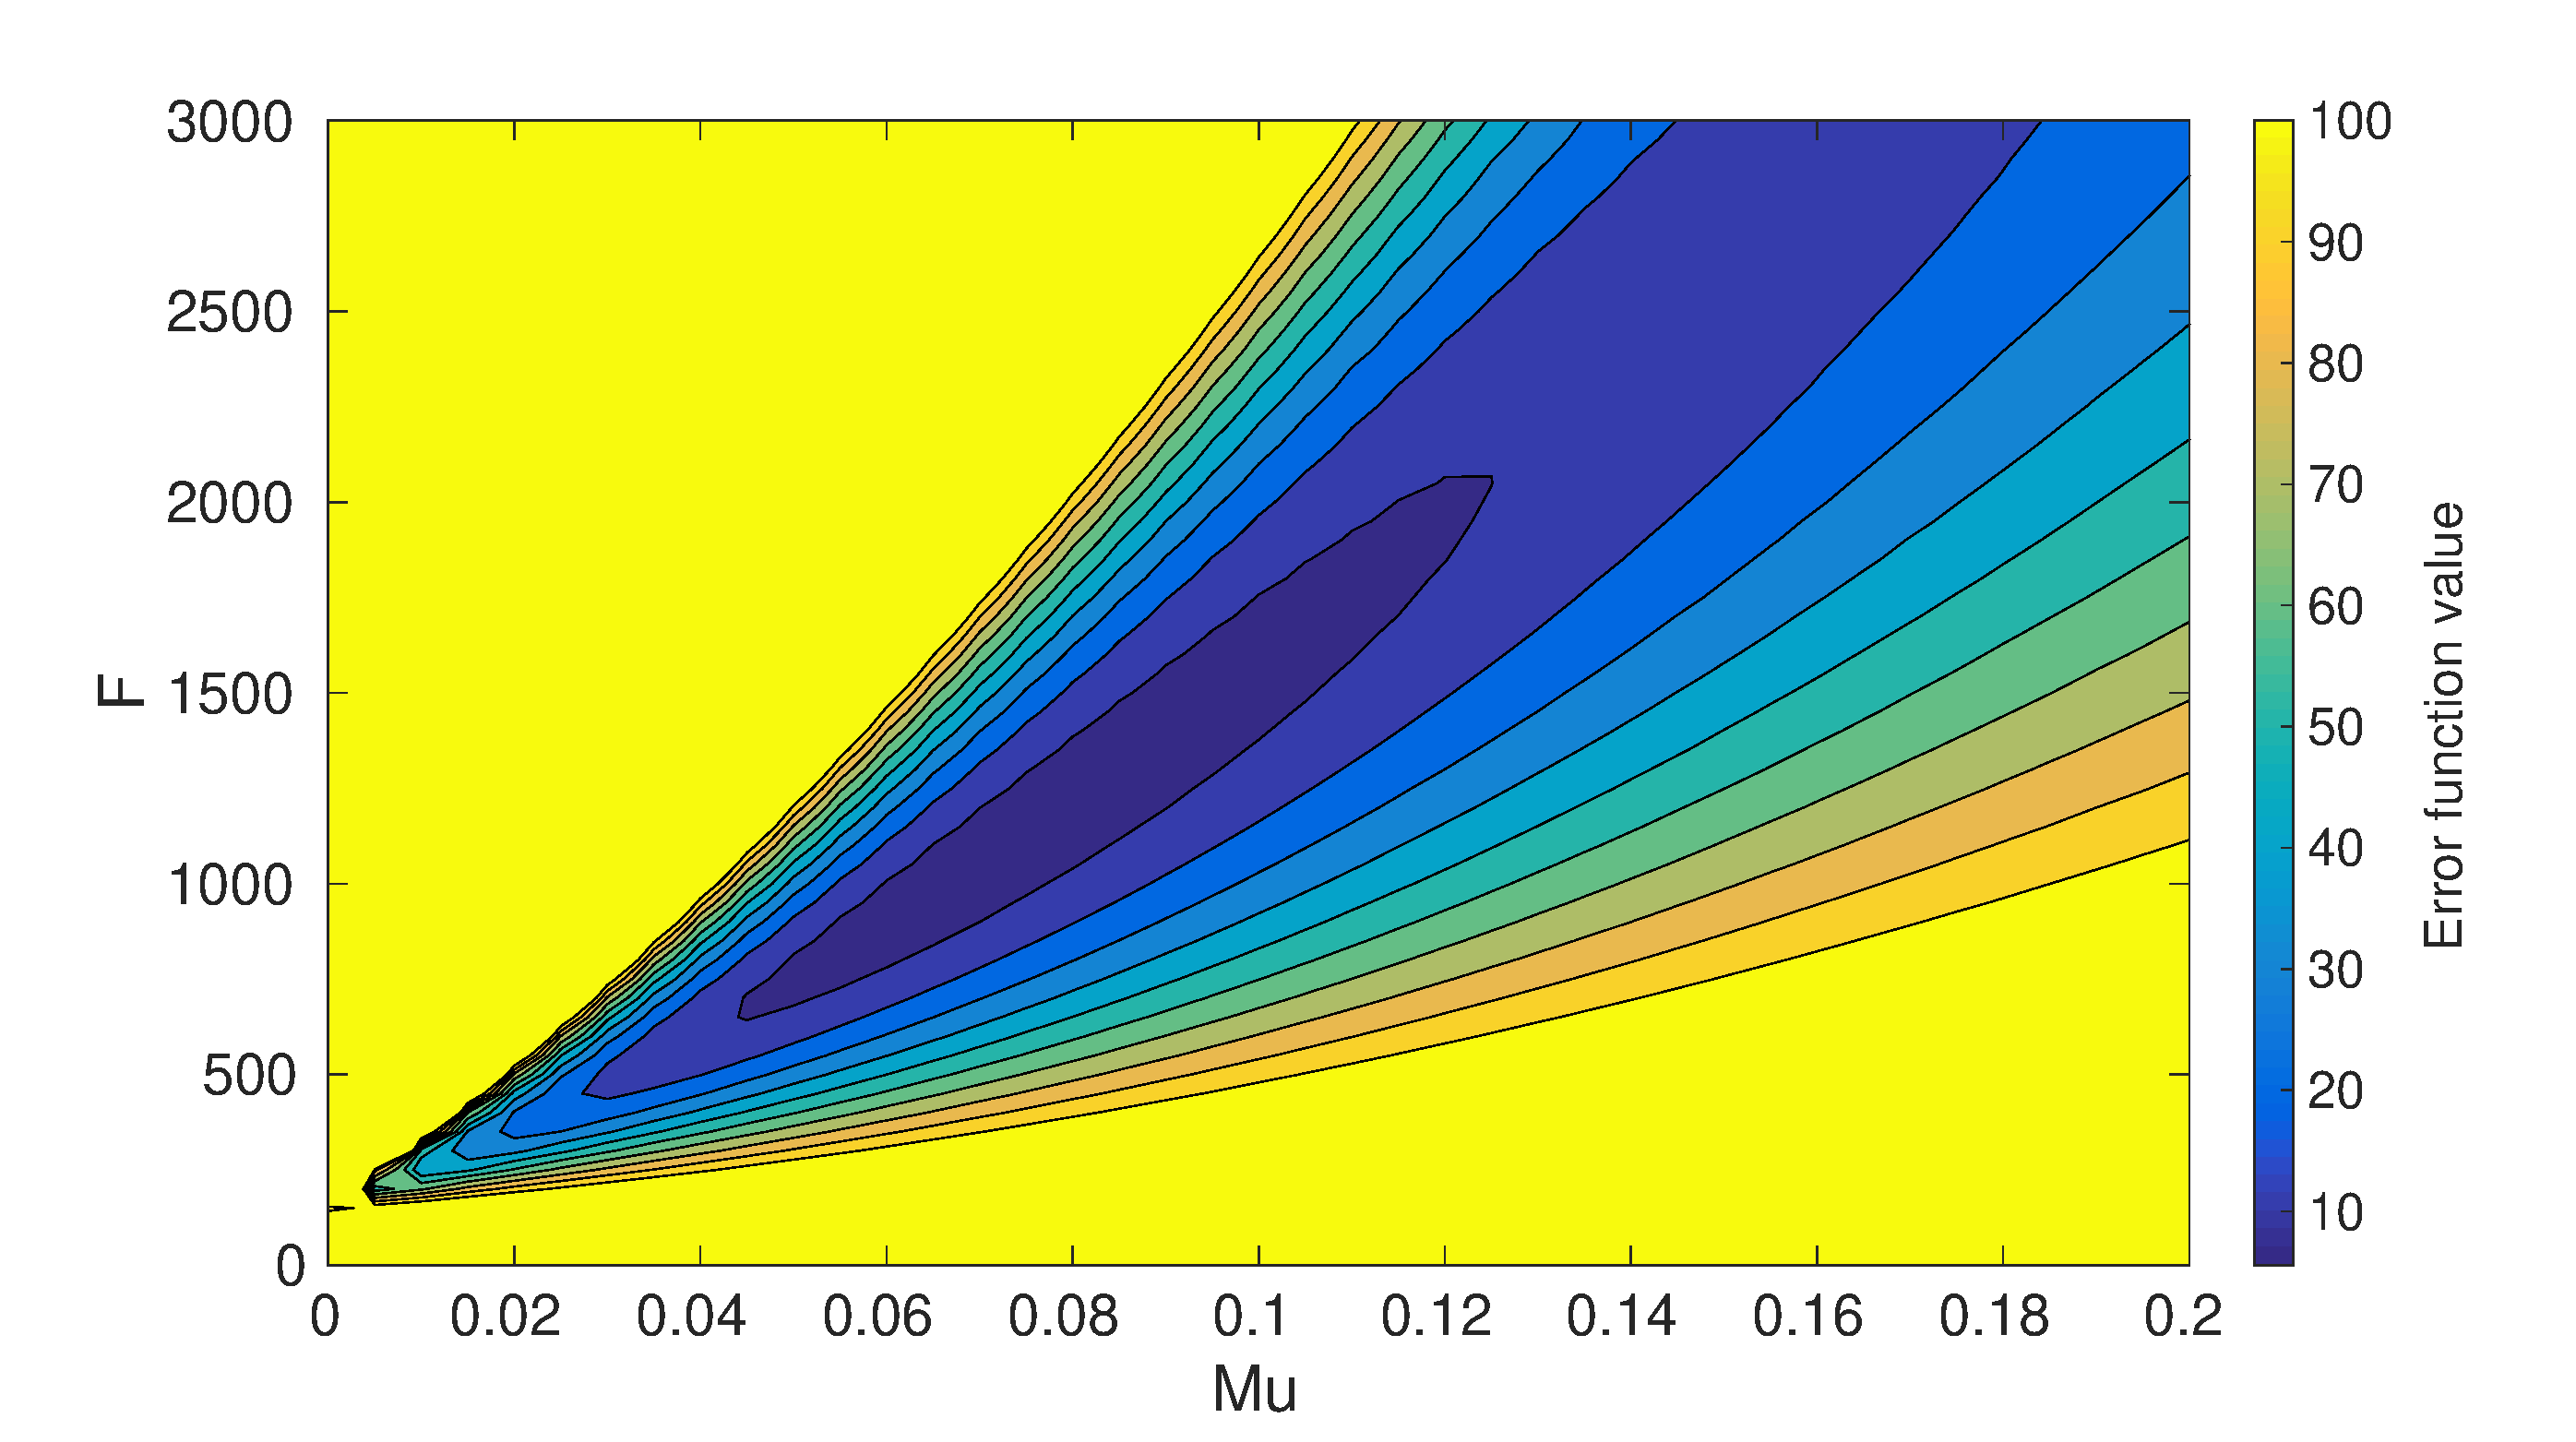
\includegraphics[scale = 0.26, clip = true, trim = 40 0 0 0]{Figures/Likelihood_rough_presentation}
    \begin{itemize}
\item  Error landscape, $\Theta = 5400$.
\end{itemize}
\end{frame}

\subsection{Future Work}


\begin{frame}{Conclusions and further work}
  \begin{itemize}
  \item Fluorescence data \alert {not enough} to estimate all unknown parameters 
  \begin{itemize}
  \item Simplified model not helpful in estimating original parameters.
  \end{itemize}
  \end{itemize}
To get these parameters ...
  \begin{itemize}
  \item Further experiments needed - observe fast timescale.
  \item Improve methodology
    \begin{itemize}
    \item Algorithms for dealing with complex chemical models \& limited data.
    \item Bayesian Methods
      \end{itemize}
  \end{itemize}
  \end{frame}
  
  \begin{frame}{Acknowledgements}
  \begin{itemize}
  \item Manish Kushawaha, Jaramillo Lab - School of Life Sciences
  \item Shenshi Shen, Boris Kisov for data.
  \item Annabelle Ballesta - Systems Biology
  \end{itemize}
  \end{frame}
    
  \begin{frame}{Additional Slides}
  \Huge
	Additional Slides
	\normalsize
  \end{frame}
  
  
\begin{frame}{Model fixed point for estimated parameters}
  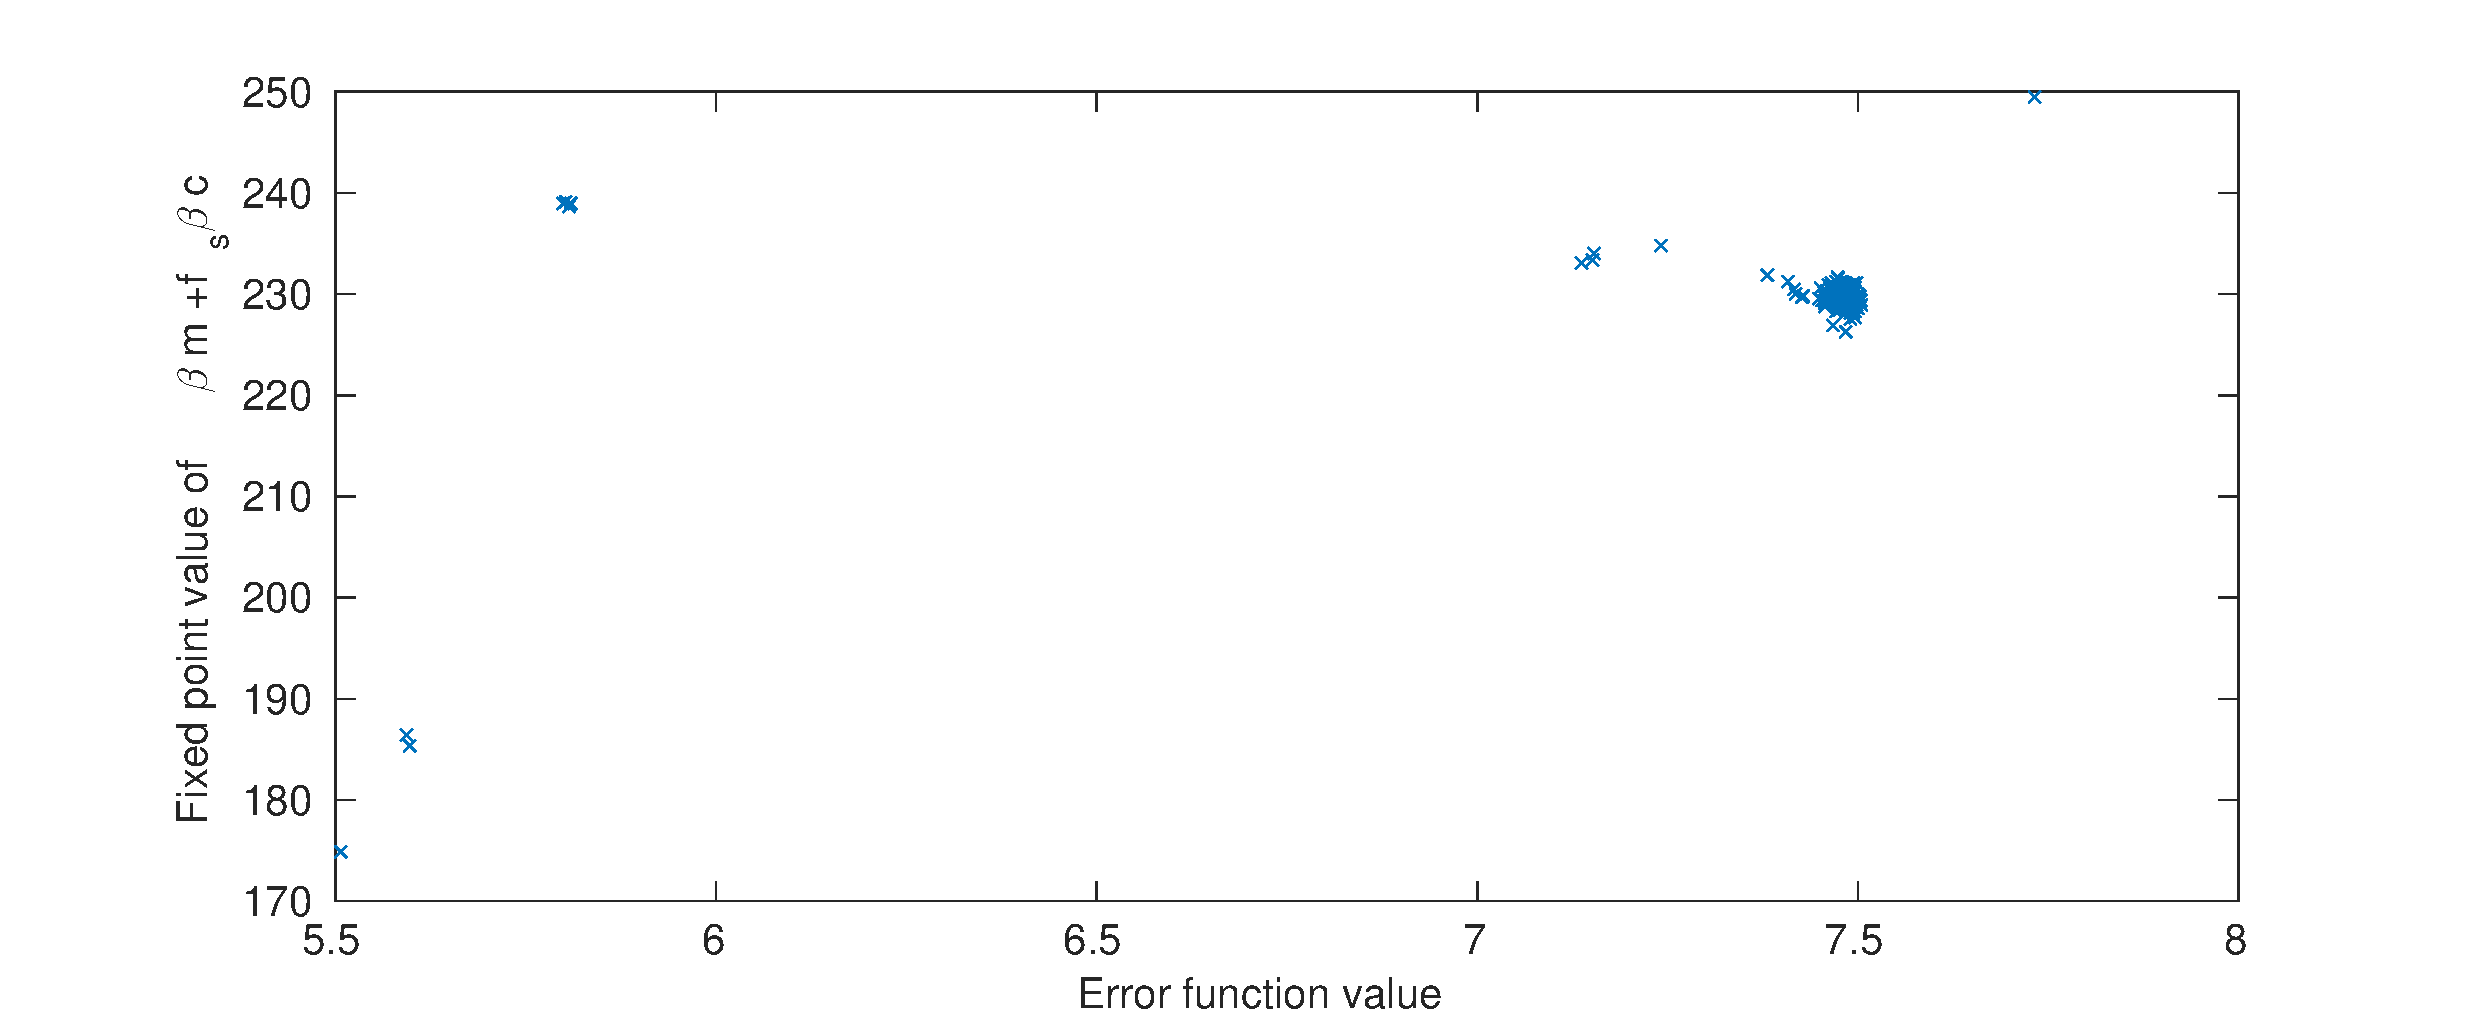
\includegraphics[scale = 0.24, clip = true, trim = 0 0 0 0]{../Figures/fixedpoint_f}
\begin{itemize}
	\item Similar fixed point values of translation forcing term, ${\beta} m +{f_{s}}\beta c$, across estimated parameter sets.
	\item Suggests translation may be rate limiting step.
\end{itemize}
\end{frame}

\end{document}





\begin{frame}{Recent Experimental Data}{}
\begin{columns}
\column{.49\textwidth}
\begin{figure}
   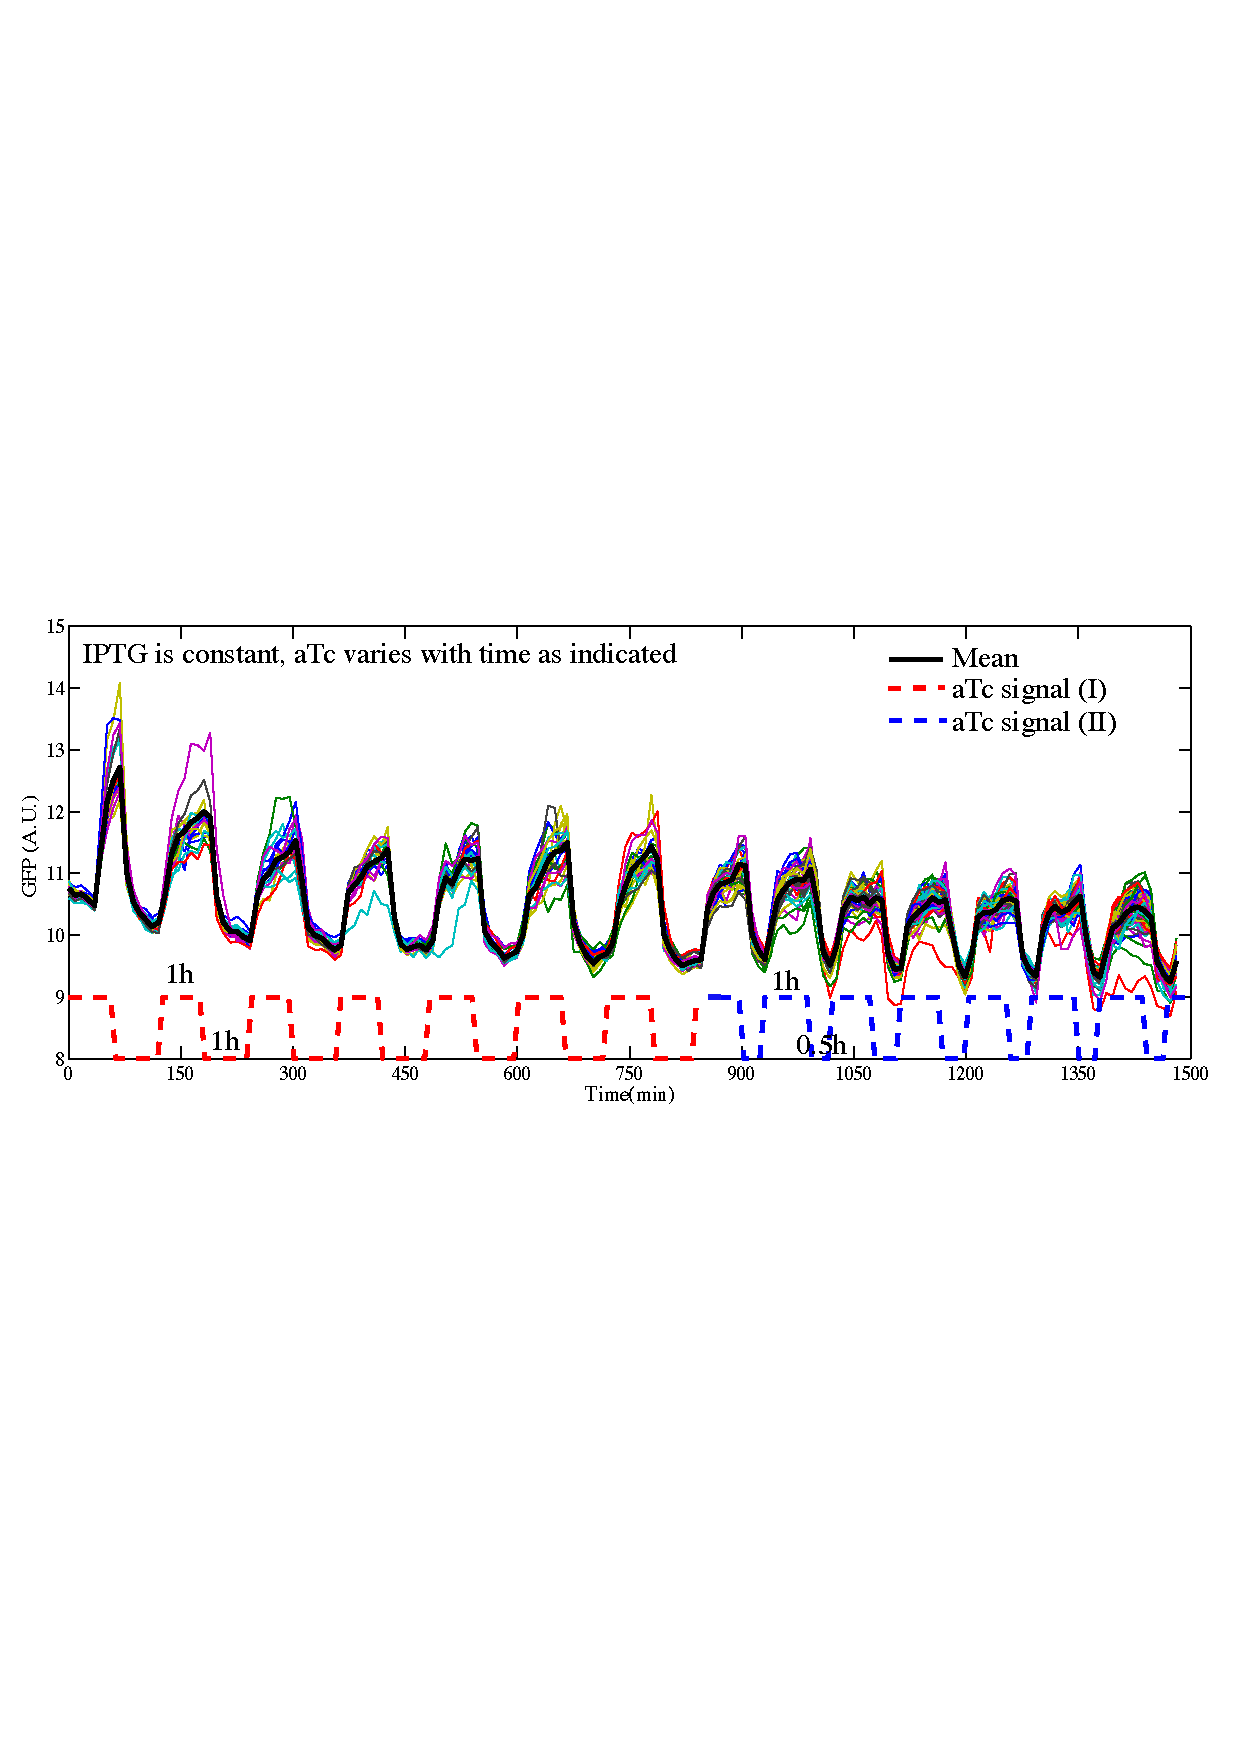
\includegraphics[trim = 10 300 270 290,clip = true,scale = 0.55]{Figures/13_9}
\end{figure}
\column{.49\textwidth}
\vspace{-5mm}
\begin{figure}
   \includegraphics[trim = 0 40 0 0 ,page=21 ,clip = true, scale=0.23]{Figures/WCPM_Warwick-talk45-220115.pdf}
\end{figure}
\end{columns}
  \begin{itemize}
    \item Single cell fluoresence time series data (Jaramillo Lab, unpublished).
    \item  Data records $z= z_{0} +\frac{g}{\alert{\Theta}} $
    \end{itemize}
\end{frame}


